\documentclass{article}

% if you need to pass options to natbib, use, e.g.:
\PassOptionsToPackage{numbers, compress}{natbib}
% before loading neurips_data_2021

% ready for submission
\usepackage{neurips_data_2021}

% to compile a preprint version, add the [preprint] option:
%     \usepackage[preprint]{neurips_data_2021}
% This will indicate that the work is currently under review.

% to compile a camera-ready version, add the [final] option:
%     \usepackage[final]{neurips_data_2021}

% to avoid loading the natbib package, add option nonatbib:
%    \usepackage[nonatbib]{neurips_data_2021}

% Submissions to the datasets and benchmarks are non-anonymous. If you do want to compile an anonymous version for other purposes, you can add the [anonymous] option:
%     \usepackage[anonymous]{neurips_data_2021}
% This will hide all author names.

\usepackage[utf8]{inputenc} % allow utf-8 input
\usepackage[T1]{fontenc}    % use 8-bit T1 fonts
\usepackage{url}            % simple URL typesetting
\usepackage{booktabs}       % professional-quality tables
\usepackage{amsfonts}       % blackboard math symbols
\usepackage{amsmath}       % blackboard math symbols
\usepackage{nicefrac}       % compact symbols for 1/2, etc.
\usepackage{microtype}      % microtypography
\usepackage[table]{xcolor}         % colors

% added by me
\usepackage{soul}           % hl
\usepackage[pdftex]{graphicx}
\usepackage{tabularx}
\usepackage[colorlinks=true,
            % linkcolor=blue,
            citecolor=black,
            urlcolor=blue,
            ]{hyperref}       % hyperlinks
\usepackage{wrapfig}
\newcolumntype{L}[1]{>{\raggedright\let\newline\\\arraybackslash\hspace{0pt}}m{#1}}
%\newcolumntype{C}[1]{>{\centering\let\newline\\\arraybackslash\hspace{0pt}}m{#1}}
%\newcolumntype{R}[1]{>{\raggedleft\let\newline\\\arraybackslash\hspace{0pt}}m{#1}}
\usepackage{tcolorbox}
\tcbuselibrary{minted,breakable,xparse,skins}

\definecolor{bg}{gray}{0.95}

% my defines
\newcommand{\figdir}{../analysis/postprocessing/figs/}

\title{Contemporary Symbolic Regression Methods and their Relative Performance}

% The \author macro works with any number of authors. There are two commands
% used to separate the names and addresses of multiple authors: \And and \AND.
%
% Using \And between authors leaves it to LaTeX to determine where to break the
% lines. Using \AND forces a line break at that point. So, if LaTeX puts 3 of 4
% authors names on the first line, and the last on the second line, try using
% \AND instead of \And before the third author name.

\author{%
        William La~Cava\footnote{corresponding author} \\
        Institute for Biomedical Informatics\\
        % Department of Biostatistics, Epidemiology and Informatics\\
        University of Pennsylvania\\
        % Philadelphia, PA 19104, USA \\
        \texttt{lacava@upenn.edu} \\
        \And
        Patryk Orzechowski \\
        Institute for Biomedical Informatics\\
        % Department of Biostatistics, Epidemiology and Informatics\\
        University of Pennsylvania\\
        % Philadelphia, PA 19104, USA \\
        \texttt{orzechowskip@upenn.edu} \\
        \And
        Bogdan Burlacu \\
        Heuristic and Evolutionary Algorithms Laboratory \\
        University of Applied Sciences \\ 
        Upper Austria Softwarepark 11, 4232 \\
        Hagenberg, Austria \\
        \texttt{Bogdan.Burlacu@fh-hagenberg.at} \\
        \And
        % Fabr\'{i}cio Olivetti de Fran\c a \\
        % F.O. de Fran\c a \\
        F.O. de Franca \\
        Center for Mathematics, Computation and Cognition, \\
        Heuristics, Analysis and Learning Laboratory \\
        Federal University of ABC \\
        Santo Andre, Brazil \\
        \texttt{folivetti@ufabc.edu.br} \\
        \And
        Marco Virgolin \\
        Mechanics and Maritime Sciences \\
        Chalmers University of Technology \\
        % Gothenburg, Sweden \\
        \texttt{ marco.virgolin@chalmers.se } \\
        \And
        Ying Jin \\
        Department of Statistics \\
        Stanford University \\ 
        % Stanford, CA 94305
        \texttt{ying531@stanford.edu} \\
        \And
        Michael Kommenda  \\
        Heuristic and Evolutionary Algorithms Laboratory \\
        University of Applied Sciences \\ 
        % Upper Austria Softwarepark 11, 4232 \\
        % Hagenberg, Austria \\
        \texttt{ michael.kommenda@fh-ooe.at }
        \And
        Jason H. Moore \\ 
        Institute for Biomedical Informatics\\
        % Department of Biostatistics, Epidemiology and Informatics\\
        University of Pennsylvania \\
        \texttt{ jhmoore@upenn.edu } \\
        % Philadelphia, PA 19104, USA \\
}

\begin{document}

\maketitle

\begin{abstract}
    % In this paper we propose a common benchmarking framework for symbolic regression, the goal of which is to unite the disparate research communities studying symbolic regression under a common set of criteria. 
Historically, the lion's share of methods for symbolic regression have relied on randomized search heuristics, especially genetic algorithms.
% Historically, symbolic regression has been tackled using randomized search heuristics, especially genetic algorithms. 
Recently, several fundamentally different approaches have been proposed, rooted in fields such as Bayesian optimization, physics, and deep learning, to name a few. 
Despite the many promising approaches to symbolic regression, progress in the field continues to suffer from a lack of consensus regarding robust benchmarking tasks, appropriate evaluation criteria, appropriate controls, and other shortcomings regarding experimental design. 
% Whereas these new approaches show promise, many of the experiments in recent work repeat common shortcomings of other symbolic regression literature, including a lack of common benchmark problems, settings, frameworks, evaluation criteria.  
In this paper, we attempt to address many of these shortcomings by proposing an open-source, reproducible benchmarking platform for symbolic regression.
% This paper describes our efforts to improve symbolic regression benchmarking standards through the design and evaluation of a common benchmarking platform called SRBench. 
% in this paper we propose SRBench, a benchmarking framework for symbolic regression.  
% to unite the disparate research communities studying symbolic regression under an 
Using this platform, we assess \hl{15} symbolic regression methods, alongside \hl{7} machine learning methods, on a set of \hl{260} different regression problems. % of varying sizes (hundreds to millions of samples). 
Our assessment includes both real-world datasets with no known model form as well as synthetic benchmark problems, including physics equations and systems of ordinary differential equations. 
For the real-world datasets, we benchmark the ability of each method to learn models with low error and low complexity relative to state-of-the-art machine learning methods. 
For the synthetic problems, we assess each method's ability to find exact solutions in the presence of varying levels of noise. 
Under these controlled experiments, we conclude that the best performing methods for real-world regression combine genetic algorithms with parameter estimation and/or semantic search drivers. 
When tasked with recovering exact equations in the presence of noise, we find that deep learning and genetic algorithm-based approaches perform similarly. 
%that recent symbolic regression methods 
% Contrary to findings from recent literature, we observe that the best performing methods for symbolic regression continue to be based in genetic algorithms, albeit with contemporary improvements. 
% The best performing methods combine genetic algorithms with recent advances in the field, including semantic backpropagation and non-linear least squares for parameter estimation.
We provide a detailed guide to reproducing this experiment and submitting new methods under continuous integration to encourage researchers to benchmark their methods using the same resource.

\end{abstract}


%%%%%%%%%%%%%%%%%%%%%%%%%%%%%%%%%%%%%%%%%%%%%%%%%%%%%%%%%%%%%%%%%%%%%%%%%%%%%%%%
\section{Introduction}
%%%%%%%%%%%%%%%%%%%%%%%%%%%%%%%%%%%%%%%%%%%%%%%%%%%%%%%%%%%%%%%%%%%%%%%%%%%%%%%%

Symbolic regression is an approach to interpretable machine learning in which the parameters, as well as the structure, of a model are optimized, typically with the goal of producing a model of a process that is easy to interpret, by virtue of its simplicity. 

Symbolic regression literature has, in general, fallen short of evaluating and/or identifying any method or family of methods that could conceivably be considered "state-of-the-art". 
In large part, these shortcomings are due to longstanding issues with the datasets used to benchmark symbolic regression, which are often small, trival, or simply not standardized (i.e. comparable) across papers or experiments~\cite{mcdermottGeneticProgrammingNeeds2012b}. 
Although community surveys~\cite{whiteBetterGPBenchmarks2012a,mcdermottGeneticProgrammingNeeds2012b} have led to suggestions for improving benchmarking standards, and even black-listed certain problems, contemporary literature continues to be published based on those datasets~\cite{petersenDeepSymbolicRegression2020}.
Furthermore, there is a stunning lack of cross-pollination between the research communities interested in symbolic regression, which include evolutionary computation, physics, engineering, statistics, and more traditional machine learning disciplines. 
Finally, lack of consensus on what SR methods constitute "state-of-the-art" is due in part to the ways in which methodological studies may be conducted - i.e., the relative merit of conducting incremental ablation studies versus large benchmark studies, such as this one. 
Whatever the causes, the result is that promising directions for future research in symbolic regression, and the outcomes that are possible, are not well supported by empirical evidence. 


The aspects of performance assessment for symbolic regression differ from typical regression benchmarking in important ways. 
For one, the competing objectives of accuracy and simplicity must be considered simultaneously.  
Furthermore, simplicity is itself a proxy for \textit{interpretability} - in other words, simplicity is often a necessary but not sufficient condition for interpretation.  
In this light, datasets with ground truth solutions are useful, in that they allow researchers to assess whether or not the symbolic model regressed by a given method is the exact solution. 
Assessing whether the symbolic model returned by a model is an exact match is non-trivial, and requires symbolic solvers with simplification procedures.
In addition, relative fidelity of estimated model forms that are not exact matches are difficult to assess.

Synthetic datasets with ground truth solutions are not sufficient for benchmarking symbolic regression algorithms. 
Such datasets do not give an adquate view into the expected performance of the algorithm when applied to datasets whose forms are yet to be discovered. 
Because of this, we consider it essential to also evaluate the performance of SR on real-world or otherwise black-box regression problems, relative to state-of-the-art ML methods. 

In this paper, we describe a large benchmarking effort that includes a dataset repository curated for symbolic regression, as well as a benchmarking repository designed to allow methodologists to easily contribute methods. 
We incorporated 130 new datasets with ground truth forms into the Penn Machine Learning Benchmark (PMLB)~\cite{olsonPMLBLargeBenchmark2017d}, including metadata describing the underlying equations, their units, and various summary statistics. 
Furthermore, we created a symbolic regression benchmark repository called SRBench\footnote{\url{https://github.com/EpistasisLab/srbench}} and sought contributions from researchers in this area. 
Here we describe this process and the results, which consist of comparisons of \hl{15} contemporary SR methods on hundreds of regression problems. 

To our knowledge this is by far the largest and most comprehensive SR benchmark effort to date, which allows us to make claims concering current state-of-the-art methods for SR with better certainty. 
Importantly, and in contrast to many previous efforts, the datasets, methods, benchmarking code, and results are completely open-source, reproducible, and revision-controlled, which should allow SRBench to exist as a living benchmark for future studies.

% New methods research risks falling into the trap of poor benchmarking strategies that have plagued previous symbolic regression efforts. 

%%%%%%%%%%%%%%%%%%%%%%%%%%%%%%%%%%%%%%%%%%%%%%%%%%%%%%%%%%%%%%%%%%%%%%%%%%%%%%%%
\section{Background and Motivation}
%%%%%%%%%%%%%%%%%%%%%%%%%%%%%%%%%%%%%%%%%%%%%%%%%%%%%%%%%%%%%%%%%%%%%%%%%%%%%%%%

\citet{kozaGeneticProgrammingProgramming1992a} introduced SR as an application of \textit{genetic programming} (GP), a field that investigates the use of genetic algorithms (GAs) to evolve executable data structures, i.e. programs. 
In the case of so-called ``Koza-style" GP, the programs to be optimized are syntax trees consisting of functions/operations over input features and constants. 
The earliest versions of GP used roulette-wheel selection to choose parents, and subtree mutation and subtree crossover to produce new variants (i.e. offspring) for the subsequent generation. 
Most SR research to date has emerged from within this subfield and its associated conferences (Genetic and Evolutionary Computation Conference (GECCO), )

Several recent works have proposed entirely different methods for tackling the SR problem. 
These include SR methods based in Bayesian optimization~\cite{jinBayesianSymbolicRegression2020}, recurrent neural networks (RNNs)~\cite{petersenDeepSymbolicRegression2020}, and physics-inspired divide-and-conquer strategies~\cite{udrescuAIFeynmanPhysicsInspired2020,udrescuAIFeynmanParetooptimal2020}. 

%% Eureqa, what it is and isn't
Some of these recent of these papers refer to Eureqa~\cite{schmidtDistillingFreeformNatural2009b}, a GP-based SR method used to re-discover known physics equations, as the "gold standard" for SR~\cite{petersenDeepSymbolicRegression2020} and/or the best method for SR "by far"~\cite{udrescuAIFeynmanPhysicsInspired2020}. 
On the basis of this claim, the aformentioned works present methods that out-perform Eureqa in terms of their ability to discover exact symbolic solutions to synthetic benchmark problems. 
However, \citet{schmidtDistillingFreeformNatural2009b} makes no claim to being the state-of-the-art method for SR, nor is this hypothesis tested in their study; in fact it is not the focus of any of the body of work on which it is based~\cite{schmidtMachineScienceAutomated2011}.  
Instead, Eureqa's development is rooted in a number of ablation studies, i.e. studies in which incremental algorithmic changes are presented and tested in controlled comparisons. 

The ``state-of-the-art" claim notwithstanding, Eureqa is certainly the most well-known and perhaps most commercially successful method for SR. 
Eureqa is a closed-source commercial software that was acquired by DataRobot in 2017\footnote{\url{https://www.datarobot.com/nutonian/}}. 
Due to its proprietary nature and incorporation into the DataRobot platform, it is impossible to benchmark its performance while controlling for important experimental variables such as computational effort. 
However, the algorithmic aspects of Eureqa are described in literature and summarized here. 
First is its use of directed acyclic graphs for representing equations in lieu of trees, which resulted in more space-efficient encodings without a significant difference in performance~\cite{schmidtComparisonTreeGraph2007}. 
The most significant improvement over traditional tournament-based selection is Eureqa's use of age-fitness Pareto optimization (AFP), a method in which random restarts are incorporated each generation as new offspring, and are protected from competing with older, more fit equations by including age as an objective to be minimized~\cite{schmidtAgefitnessParetoOptimization2011}. 
Eureqa also includes the co-evolution of fitness predictors, in which fitness assignment is sped up by optimizing a second population of training sample indices that best distinguish between equations in the population~\cite{schmidtCoevolutionFitnessPredictors2008}.
It is also possible that Eureqa no longer uses any of these reported algorithms for SR, due to its closed-source nature.
In that light, it is not clear what fundamental insight is gained when comparing to the software itself, other than a head-to-head comparison, since methodological insights cannot be extracted.

% New methods for symbolic regression
A close reading of SR literature since 2009 implies that a number of proposed methods would outperform Eureqa in controlled tests.
For one, AFP optimization has been outperformed by a number of semantic-aware selection methods (e.g.,~\cite{lacavaEpsilonLexicaseSelectionRegression2016c,liskowskiDiscoverySearchObjectives2017}), some of which are included in our study, alongside AFP.
Many other lines of research have pointed in promising directions, including hybridizations of GP with local search for constant optimization~\cite{topchyFasterGeneticProgramming2001,kommendaParameterIdentificationSymbolic2019} or structural tuning~\cite{lacavaInferenceCompactNonlinear2016}; the increasing use of semantic methods for guiding variation~\cite{moraglioGeometricSemanticGenetic2012a,virgolinLinearScalingSemantic2019} and selection~\cite{azadKrzysztofKrawiecBehavioral2017,lacavaProbabilisticMultiobjectiveAnalysis2019,arnaldoMultipleRegressionGenetic2014a}; and alternative representations of equations~\cite{defrancaInteractionTransformationEvolutionaryAlgorithm2020,mcconaghyFFXFastScalable2011}.

% lack of standards in symbolic regression field
The widespread adoption of these promising SR approaches is ham-strung by a lack of consensus on good benchmark problems, testing frameworks, and experimental designs. 
Our effort to establish a common benchmark is motivated by our view that the lack of strong, standardized benchmarks in the SR community impedes the adoption of promising techniques and impedes progress.  
As a counterexample, consider the comparatively quick adoption of advances in the neural network community that create a ratcheting effect of progress towards better methods and architectures. 
The quicker adoption of advancements for NNs is partially explained by the community's size, but we would contend that it is also due in part to community-wide focus on common benchmarks, frameworks (e.g. TensorFlow, PyTorch) and experiment designs. 
In comparison, in SR literature it is common to publish results on a small number of small, easy, and unrealistic problems, comparing only to very basic GP systems such as those described in~\cite{kozaGeneticProgrammingProgramming1992a} nearly thirty years ago.   
The issues around benchmarking have been described in detail~\cite{mcdermottGeneticProgrammingNeeds2012b}, and even led to community surveys and a proposal to ``black-list" several toy problems often reported in literature, such as the quartic polynomial problem~\cite{whiteBetterGPBenchmarks2012a}.
Despite these efforts to improve standards nearly ten years ago, toy datasets and comparisons to out-dated SR methods continue to appear in contemporary literature.

% efforts to benchmark SR
There have been recent efforts to improve benchmarking standards for SR.
\citet{zegklitzBenchmarkingStateoftheartSymbolic2020} benchmarked four SR methods (specifically those using linear regression) on five datasets. 
A larger benchmark (and precursor to this work) evaluated four recent SR methods on 94 regression problems in comparison to nine state-of-the-art ML approaches~\cite{orzechowskiWhereAreWe2018}. 
In both cases, SR methods were assessed solely on their ability to make accurate predictions. 
In contrast, \citet{udrescuAIFeynmanPhysicsInspired2020} proposed 120 new synthetic, physics-based datasets for SR, but compared only to Eureqa and only in terms of exact solutions. 
A major contribution of our work is its significantly more comprehensive scope than previous research.
We include \hl{15} SR methods on \hl{252} datasets in comparison to \hl{7} ML methods. 
Our comparisons are also more comprehensive: methods are benchmarked on their ability to generate models that are 1) accurate, 2) simple, and 3) exact or approximate symbolic matches to the ground truth process. 
In addition, we have made the benchmark openly available, reproducible, and open for contributions supported by continuous integration. 

% \subsection{Trends in Genetic Programming Literature}

% semantic methods

% parameter estimation 

% representation/encodings 

%%%%%%%%%%%%%%%%%%%%%%%%%%%%%%%%%%%%%%%%%%%%%%%%%%%%%%%%%%%%%%%%%%%%%%%%%%%%%%%%
\section{Methods}
%%%%%%%%%%%%%%%%%%%%%%%%%%%%%%%%%%%%%%%%%%%%%%%%%%%%%%%%%%%%%%%%%%%%%%%%%%%%%%%%

We created SRBench with the goal of having a living benchmarking of SR methods that invites rolling contributions. 
In order to establish common datasets, we extended PMLB, a standardized set of regression and classification problems\cite{olsonPMLBLargeBenchmark2017d}, by adding 130 SR datasets with known model forms. 
In order to standardize framework comparisons, we required contributors to define a minimal, Scikit-learn compatible~\cite{pedregosaScikitlearnMachineLearning2011a}, Python API for their method. 
An example contribution is shown in Figure~\ref{fig:ex_code}.

To ensure reproducibility, we defined a common environment (via conda) and with fixed versions of packages and their dependencies. 
We defined a continuous integration testing framework that tested the installation of new methods within this environment, and runs a set of tests to ensure new methods are compatible with the benchmark code.  
New contributions are submitted as pull requests and tested automatically.

We defined the experiment in two parts.
The first is a comparison of SR methods on ``black-box" regression problems, for which the metrics of interest are test set accuracy, model complexity, and training time. 
The second is a comparison of SR methods on ``ground-truth" regression problems, for which the metrics of interest are exact solution rates, test set accuracy, model complexity, and training time. 


\paragraph{Accuracy}
We assessed accuracy using the coefficient of determination ($R^2$), defined as 

\begin{equation}
    R^2 = 1 - \frac{\sum_i^N{(y_i - \hat{y}_i)^2}}
                   {\sum_i^N{(y_i - \bar{y}_i)^2}}
\end{equation}

%%
% complexity
%%
\paragraph{Complexity}
A number of different complexity measures have been proposed for SR, including those based in \textit{syntactic} complexity (i.e. related to the complexity of the symbolic model), \textit{semantic} complexity (i.e. related to the behavior of the model over the data)~\cite{vladislavlevaOrderNonlinearityComplexity2009a,udrescuAIFeynmanParetooptimal2020}, or both~\cite{kommendamichaelEvolvingSimpleSymbolic2015}. 
The pros and cons of these methods and their relation to generalization and interpretability is discussed frequently in literature~\cite{murdochDefinitionsMethodsApplications2019}. 
For the sake of simplicity, we opted to define complexity as the number of simple mathematical operators, nodes and constants in the model, where simple mathematical operators are in the set 
$\{+,
    -,
    *,
    {/},
    \sin,
    \cos,
    \arcsin,
    \arccos,
    \exp,
    \log, 
\text{pow},
\max,
\min \}$. 
In addition to calculating the complexity of the raw model forms returned by each method, we calculated the complexity of the models after simplifying via \href{https://www.sympy.org/en/index.html}{sympy}.

%%
% solutions
%%%
\paragraph{Solution Criteria}
For the ground truth regression problems, we evaluated whether the final model was a ``solution" to the task according to two metrics: \textit{accuracy solution} and \textit{symbolic solution}. 
A final model was considered an accuracy solution if it had a (near) perfect accuracy on the test set, defined as $R^2>0.999$. 
A model was considered a symbolic solution if it was non-constant and satisifed at least one of the following conditions: 

\begin{enumerate}
    \item $\phi^*-\hat{\phi} = c $
    \item $\frac{\phi^*}{\hat{\phi}} = c $ 
\end{enumerate}

where $c$ is a constant. 
This definition is designed to capture models within an affine transformation of the true model form (those that differ only by a constant or scalar). 
Prior to assessing symbolic solutions, each model underwent sympy simplification, as did the conditions above. 
We chose to report both of these solution definitions because there are pros and cons to both. 
Symbolic solutions are preferable to accuracy solutions in the sense that they are more a more faithful evaluation of the ability of an SR method to discover the data generating process.
However, because any symbolic function can be represented in an infinite number of ways, and sympy's simplification procedure uses non-optimal heuristics, we cannot guarantee that all symbolic solutions are captured with perfect fidelity by this metric. 
The accuracy solution metric more explicitly measures the model's ability to perfectly capture the underlying process, yet it has the disadvantage of being reported over finite samples. 
Therefore accuracy solutions may not truly capture the data generating process. 
In this sense, one may view the accuracy solution and symbolic solution metrics as optimistic and pessimistic estimates of performance, respectively.

\subsection{Symbolic Regression Methods}

We evaluated a number of SR algorithms in this benchmark that are summarized in Table~\ref{tbl:methods}.
Here we briefly describe what these methods are and describe how they fit into broader research trends within the SR field. 

% table of methods
\begin{table}
    \footnotesize
    \center
    \caption{
        Short descriptions of the SR methods benchmarked in our experiment, including references and links to implementations. 
    }\label{tbl:methods}
    \rowcolors{2}{gray!25}{white}
    \begin{tabular}{l L{12em} L{8em} r}
        \rowcolor{white}
        Method      &   Description                                         &   Method Family                       &   Implementation  \\ 
        \midrule
        AFP~\cite{schmidtAgefitnessParetoOptimization2011}               &   Age-fitness Pareto Optimization     &   GP
                    &   C++/Python (\href{https://github.com/EpistasisLab/ellyn}{link})                  \\
        AIFeynman~\cite{udrescuAIFeynmanParetooptimal2020}               &   Physics-inspired method             &   Divide and conquer
                    &   Fortran/Python (\href{https://github.com/SJ001/AI-Feynman}{link})              \\
        BSR~\cite{jinBayesianSymbolicRegression2020}                     &   Bayesian Symbolic Regression        &   Markov Chain Monte Carlo
                    &   Python (\href{https://github.com/ying531/MCMC-SymReg}{link})                      \\
        DSR~\cite{petersenDeepSymbolicRegression2020}                    &   Deep Symbolic Regression            &   Recurrent neural networks   
                    &   Python (PyTorch) (\href{https://github.com/brendenpetersen/deep-symbolic-regression}{link})            \\
        EPLEX~\cite{lacavaProbabilisticMultiobjectiveAnalysis2019}       &   $\epsilon$-lexicase selection       &   GP
                    &   C++/Python (\href{https://github.com/EpistasisLab/ellyn}{link})                  \\
        FEAT~\cite{lacavaLearningConciseRepresentations2019c}        &   Feature Engineering Automation Tool &   GP                          
                    &   C++/Python (\href{https://github.com/lacava/feat}{link})                  \\
        AFP\_FE~\cite{schmidtDistillingFreeformNatural2009b}               &   AFP with co-evolved fitness estimates; Eureqa-esque     &   GP
                    &   C++/Python (\href{https://github.com/EpistasisLab/ellyn}{link})                  \\
        FFX~\cite{mcconaghyFFXFastScalable2011}         &   Fast function extraction             &   Random search               
                    &   C++/Python (\href{https://github.com/natekupp/ffx/tree/master/ffx}{link})                  \\
        GPGOMEA~\cite{virgolin2020improving}     &   Gene-pool Optimal Mixing Evolutionary Algorithm     & GP            
                    &   C++/Python (\href{https://github.com/marcovirgolin/GP-GOMEA/}{link})                  \\
        gplearn     &   Koza-style symbolic regression in Python       &   GP                          
                    &   C++/Python (\href{https://github.com/trevorstephens/gplearn}{link})                  \\
        ITEA~\cite{defrancaInteractionTransformationEvolutionaryAlgorithm2020}   &   Interaction-Transformation EA       &   GP
                    &   Haskell/Python (\href{https://github.com/folivetti/ITEA/}{link})              \\
        MRGP~\cite{arnaldoMultipleRegressionGenetic2014a}                        &   Multiple Regression Genetic Programming &   GP
                    &   Java (\href{https://github.com/flexgp/gp-learners}{link})                        \\
        Operon~\cite{kommendaParameterIdentificationSymbolic2019}                &   SR with Non-linear least squares     &   GP
                    &   C++/Python (\href{https://github.com/heal-research/operon}{link})                  \\
        SemBackProp~\cite{virgolinLinearScalingSemantic2019}                     &   Semantic Back-propagation           &   GP
                    &   C++/Python (\href{https://github.com/marcovirgolin/GP-GOMEA}{link})                  \\ 
        \bottomrule
    \end{tabular}
\end{table}



% \subsubsection{Genetic Programming-Based Methods}
% Most methods for SR come from the genetic programming (GP) literature. 
The canonical implementation of GP-based SR starts with an initially random population programs/models, and then iterates through the steps of selection, variation and (optionally) survival~\cite{poliFieldGuideGenetic2008}.
Selection chooses individuals from which to produce new points in the search space in the subsequent iteration. 
The de-facto method of selection is tournament selection, in which a fixed-size sample of individuals are drawn and the fittest individual chosen as winner. 
Selected models then under-go some combination of randomized mutation and/or crossover, traditionally at the subtree level or single node level.
In Koza-style GP, the resulting offspring replace the parents, but several common methods include a survival step in which the resulting offspring compete against the parents, at the very least to ensure the best model in the search space is not lost.
This canonical method of GP-based SR is embodied by \textbf{gplearn}. 
With these basic components in mind, we briefly describe the contemporary methods listed in Table~\ref{tbl:methods} based on the steps which they target - i.e. selection/survival, variation/recombination, fitness/evaluation, or program representations. 

\paragraph{Pareto Optimization}

An established approach to optimizing the accuracy and simplicity of candidate equations is to use multi-objective optimization methods such as NSGA-II\hl{cite} and SPEA-II\hl{cite}. 

\textbf{AFP}

\textbf{FE\_AFP} is an implementation that closely mirrors key aspects of Eurequa as desribed in literature. 

\paragraph{Semantic Search Drivers}

Another promising line of research has been to leverage program \textit{semantics} (in this case, the equation's intermediate and final outputs over all training samples) more heavily during the stages of selection, variation and survival. 
When a program's semantics are collapsed into single aggregate fitness values during optimization, an "information bottleneck" is created in which potentially valuable information about building blocks in the problem space, as well as the program space, is lost~\cite{azadKrzysztofKrawiecBehavioral2017}. 

One selection that has emerged as an improvement over tournament selection and AFP is $\epsilon$-lexicase selection (\textbf{EPLEX})~\cite{lacavaEpsilonLexicaseSelectionRegression2016c}. 
Rather than aggregating the training loss across samples, EPLEX utilizes the error vectors to conduct selection as if through a series of filters. 
We benchmark EPLEX as a stand-alone change, but it also appears as the parent selection method in FEAT~\cite{lacavaLearningConciseRepresentations2019c}. 

Semantic backpropagation (\textbf{SBP}) is a technique invented and popularized by~\cite{wieloch2013running,krawiec2013approximating,pawlak2014semantic} to compute, for a given target value and a tree node position, what output is needed at the given position to make the output of the tree match the target value. 
It works by iterative inversions of the ancestry of function nodes, from the root down to the chosen node position. 
Here, we rely on the algorithm by~\citet{virgolinLinearScalingSemantic2019}, an SBP -based GP which is capable to tackle real-world regression datasets. 
In this algorithm, similarly to~\cite{wieloch2013running}, recombination improves a solution by applying SBP on a random node position and using the label as target, and replacing the subtree rooted at the sampled position with a tree chosen from a pre-computed library. 
The chosen tree has output that best matches the one computed by SBP (i.e., using the Euclidean distance on output vectors defined over the training set). 
Moreover, optimal affine transformations are computed at the start of SBP and during library parsing, resulting in substantial performance gains~\cite{virgolinLinearScalingSemantic2019}.

\paragraph{Constant optimization}

Traditional GP encodes constants as building blocks that are initialized from a given distribution, and then optimizes them through the same process as the rest of the component building blocks.
One of the clearest improvements over Koza-style GP has been the adoption of local search methods to handle constant optimization distinctly from evolutionary learning. 
Backpropagation-based gradient descent has been proposed for GP-SR by~\citet{topchyFasterGeneticProgramming2001}, but for years was not widely adopted. 
For example, the methods of~\citet{bongardNonlinearSystemIdentification2005a} and~\citet{schmidtDistillingFreeformNatural2009} that would appear years later opted for stochastic hill climbing for handling constant optimization. 
More recent studies~\cite{kommenda_effects_2013,kommendaParameterIdentificationSymbolic2019} have made a strong case for the use of non-linear least squares approaches to constant optimization, and establish gradient-based constant optimization as an improvement over stochastic and evolutionary approaches.
The aformentioned studies are embodied by \textbf{Operon}, a GP method that incorporates non-linear least squares constant optimization using the Levenberg-Marquadt algorithm\cite{burlacuOperonEfficientGenetic2020}.

\paragraph{Equation Encodings}

In addition to the question of how to best optimize constants, a line of research has proposed improved ways of defining constants within or between program encodings. 
Rather than treating constants as building blocks, FEAT~\cite{lacavaLearningConciseRepresentations2019c} and \textbf{Operon}~\cite{burlacuOperonEfficientGenetic2020} encode weights at the edges of all nodes. 
\textbf{MRGP}~\cite{arnaldoMultipleRegressionGenetic2014a} splays individual program stack trace out as a matrix, using Lasso to identify building blocks and to train the final model.
Methods such as \textbf{FFX}~\cite{mcconaghyFFXFastScalable2011}, EFS~\cite{arnaldoBuildingPredictiveModels2015}, and FEW~\cite{lacavaGeneralFeatureEngineering2017} treat the entire population as a single model for which individuals are features.

\textbf{ITEA}

\paragraph{Gene-pool Optimal Mixing Evolutionary Algorithm}

The Genetic Programming version of the Gene-pool Optimal Mixing Evolutionary Algorithm (GP-GOMEA) is an EA with adaptive recombination based on a \emph{linkage model}~\cite{virgolin2017scalable,virgolin2020improving}. 
A linkage model is a model of the level of interdependencies (i.e., linkage) existing within the encoding of evolving solutions~\cite{thierens2011optimal}. 
Like other algorithms of the GOMEA family, GP-GOMEA computes a linkage model every generation, and uses this information to guide its recombination phase. 
The goal is to prevent the disruption potentially-salient patterns of components, i.e., \emph{building blocks} with a positive concerted action.
In~\cite{virgolin2017scalable,virgolin2020improving}, it was shown that GP-GOMEA’s linkage-based recombination works significantly better than random recombination, and is especially competitive when small, potentially interpretable solutions are sought. 
We use the same implementation of~\cite{virgolin2020improving}.

\paragraph{Bayesian Symbolic Regression}

\citet{jinBayesianSymbolicRegression2020} recently proposed Bayesian Symbolic Regression (BSR), in which a prior is placed on tree structures and the posterior distributions are sampled using a Markov Chain Monte Carlo (MCMC) method.   
As in GP-based SR, arithmetic expressions are expressed with symbolic trees, although BSR explicitly defines the final model form as a linear combination of several symbolic trees. 
Model parsimony is encouraged by specifying a prior that presumes additive, linear combinations of small components. 

\paragraph{Deep Symbolic Regression}
Deep Symbolic Regression (\textbf{DSR})~\cite{petersenDeepSymbolicRegression2020} uses a recurrent neural network architecture and reinforcement learning, including a novel a risk-seeking policy gradient. 
DSR showed good performance in finding exact solutions to a number of synthetic benchmark problems, although 6 of the 12 problems for which they reported results in the main text (c.f. Table 1,~\cite{petersenDeepSymbolicRegression2020}) are low-order synthetic polynomials that were proposed for black-listing in community surveys (c.f. Table 3, \citet{whiteBetterGPBenchmarks2012a}).  

\paragraph{AI-Feynman}
\hl{TODO}

%%%%%%%%%%%%%%%%%%%%%%%%%%%%%%%%%%%%%%%%%%%%%%%%%%%%%%%%%%%%%%%%%%%%%%%%%%%%%%%%
\section{Experimental Setup}
%%%%%%%%%%%%%%%%%%%%%%%%%%%%%%%%%%%%%%%%%%%%%%%%%%%%%%%%%%%%%%%%%%%%%%%%%%%%%%%%

We evaluated SR methods on two separate tasks. 
First, we assessed their ability to make accurate predictions on "black-box" regression problems while minimizing the syntactic complexity of the solution. 
Here "black-box" refers to not knowing the functional form of the underlying data-generating process, assuming one exists.   
Second, we tested the ability of each method to find exact solutions to synthetic datasets with known, ground-truth functions. 
The second set of problems are based on physics equations from several sources, as described below. 

The basic experiment settings are summarized in Table~\ref{tbl:exp}.
Each algorithm was trained on each dataset (and level of noise, for ground-truth problems) in 10 repeated trials with a different random state that controlled both the train/test split and the seed of the algorithm.  
Datasets were split 75/25\% in training and testing. 
For black-box regression problems, each algorithm was tuned using 5-fold CV with halving grid search. 
The SR algorithms were limited to 6 hyperparameter combinations; the ML methods were allowed more, as shown in Appendix Tables~\ref{tbl:ml_methods}-\ref{tbl:sr_methods2}. 
The best hyperparameter settings were used to tune a final estimator and evaluate it according to the metrics described above. 
Details for running the experiment are given in the Appendix. 

\begin{table}
    \footnotesize
    \center
    \caption{
        Settings used in the benchmark experiments. 
        ``Total comparisons" refers to the total evaluatons of an algorithm on a dataset for a given noise level and random seed.
    }\label{tbl:exp}
    % \rowcolors{2}{gray!25}{white}
    \begin{tabular}{lll}
        Setting                     &   Black-box Problems              &   Ground-truth Problems                   \\
        \midrule
        No. of datasets             &   122                             &   130                                     \\
        No. of algorithms           &   21 (14 SR, 7 ML)                &   14                                      \\
        No. of trials per dataset   &   10                              &   10                                      \\
        Train/test Split            &   .75/.25                         &   .75/.25                                 \\
        Hyperparameter Tuning       &   5-fold Halving Grid Search CV   &   None (best set from BB problems)        \\
        Termination criteria        &   500k evaluations/train or 48 hours    &   1M evaluations or 8 hours         \\ 
        Levels of target noise      &   None                            &   0, 0.001, 0.01                          \\
        Total comparisons           &   26840                           &   54600                                   \\ 
        \bottomrule
    \end{tabular}
\end{table}


\subsection{Black-box Regression Problems}

We used \hl{122} black-box regression problems available in PMLB v.1.0. 
These problems are pulled from, and overlap with, varous open-source repositories, including OpenML~\cite{vanschorenOpenMLNetworkedScience2013} and the UCI repository~\cite{lichmanUCIMachineLearning2013a}. 
PMLB standardizes these datasets to a common format and provides fetching functions to load them into Python (and R). 
Each dataset includes metadata describing source information as well as a profile detailing the data distributions (e.g. \href{https://epistasislab.github.io/pmlb/profile/analcatdata_aids.html}{this dataset}).

\subsection{Ground-Truth Regression Problems}
We extended PMLB with 130 datasets with known, ground-truth model forms. 
These datasets were used to assess the ability of SR methods to recover known process physics. 
The 130 datasets came from two sources: the \href{https://space.mit.edu/home/tegmark/aifeynman.html}{Feynman Symbolic Regression Database}, 
and the \href{https://github.com/lacava/ode-strogatz}{ODE-Strogatz repository}.

Both sets of data come from first principles models of physical systems. 
The Feynman problems originate in the \textit{Feynman Lectures on Physics}\cite{feynmanFeynmanLecturesPhysics2015}, and the datasets were recently created and proposed as SR benchmarks~\citet{udrescuAIFeynmanPhysicsInspired2020}. 

Whereas the Feynman datasets represent static systems, the Strogatz problems are non-linear and chaotic dynamical processes~\cite{strogatzNonlinearDynamicsChaos2014}.
Each dataset is one state of a 2-state system of first-order, ordinary differential equations (ODEs). 
They were used to benchmark SR methods in previous work~\cite{lacavaInferenceCompactNonlinear2016,schmidtMachineScienceAutomated2011}.

%%%%%%%%%%%%%%%%%%%%%%%%%%%%%%%%%%%%%%%%%%%%%%%%%%%%%%%%%%%%%%%%%%%%%%%%%%%%%%%%
\section{Results}
%%%%%%%%%%%%%%%%%%%%%%%%%%%%%%%%%%%%%%%%%%%%%%%%%%%%%%%%%%%%%%%%%%%%%%%%%%%%%%%%
The median test set performance on all problems and methods for the black-box benchmark problems is summarized in Figure~\ref{fig:pmlb_perf}. 
Among all methods, we observe the best test set performance using Operon. 

The top three methods (Operon, SBP, FEAT) are all GP based SR methods. 
Not only do they outperform other SR methods, they also perform on par or better than state-of-the-art ML methods like XGB and LGBM. 
\hl{todo: stats}. 

Across problems, DSR and BSR do not perform significantly different from penalized linear regression (Linear). 
DSR also has the third longest running time. 

AIFeynman performs poorly on these problems, suggesting that not many of them exhibit the qualities of physics systems (translatability, symmetry, etc) that AIFeynman was designed to exploit. 

\hl{add stats table}

Performance on the ground-truth regression problems is summarized in Figure~\ref{fig:symbolic_solns}. 
Methods are sorted by their solution rate for the middle level of noise (0.001). 
We observe that, as in previous literature, AIFeynman performs well in terms of finding exact solutions for systems without noise. 
However, we found AIFeynman to be quite sensitive to added noise. 
In contrast, FE\_AFP, DSR perform similarly well (with a minor drop in success rate) as noise is added, suggesting they are would be less brittle in application to real-world data. 

We note that the best method on real-world data, Operon, here struggles to recover symbolic solutions to these problems, despite also finding many candidate solutions with perfect or near prefect test set scores (center panel, Figure~\ref{fig:symbolic_solns}. 
We see a similar pattern with MRGP, and also note that MRGP exhibits overfitting to the addition of noise, as noted by the larger final model sizes it produces. 

% \subsection{Black-box Regression Problems}
% overall pmlb results
\begin{figure}
    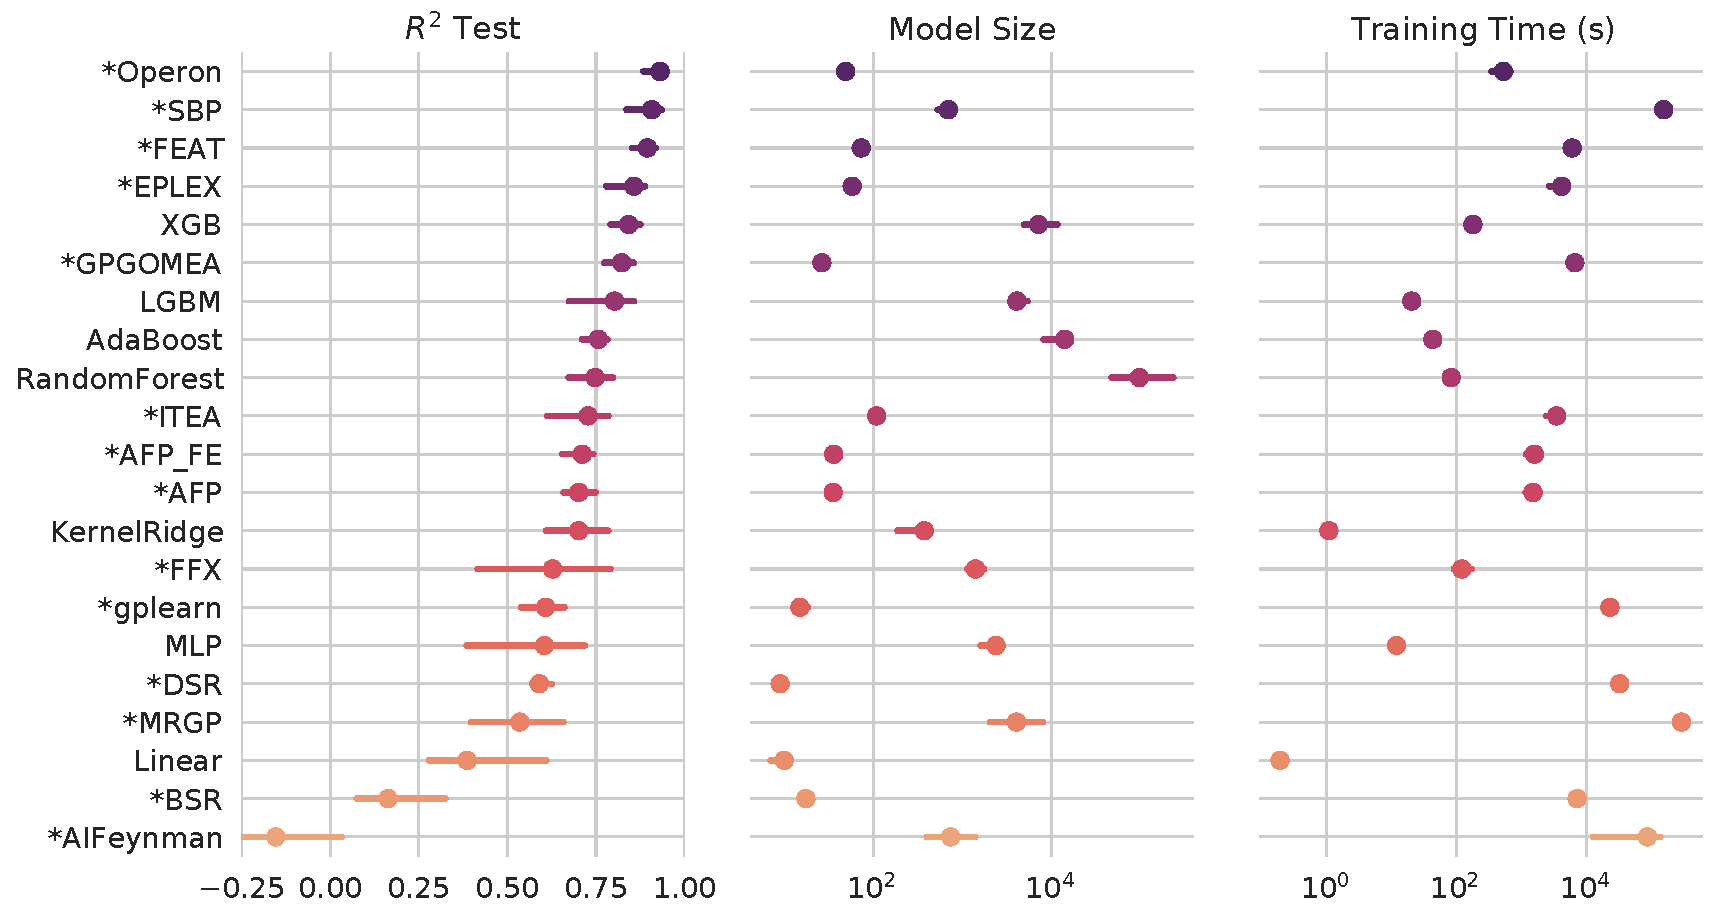
\includegraphics[width=\textwidth]{figs/results_pmlb_r1/pairgrid-pointplot_r2_test_model_size_training-time-(s).pdf}
    \caption{ 
        Results on the black-box regression problems.
        Points indicate the mean of the median test set performance on all problems, and bars show the 95\% confidence interval. 
        Methods marked with an asertisk are SR methods. 
    }
    \label{fig:pmlb_perf}
\end{figure}

% \subsection{Ground-Truth Regression Problems}
% solutions in terms of perfect accuracy, perfect models
% success rates

\begin{figure}
    \centering
    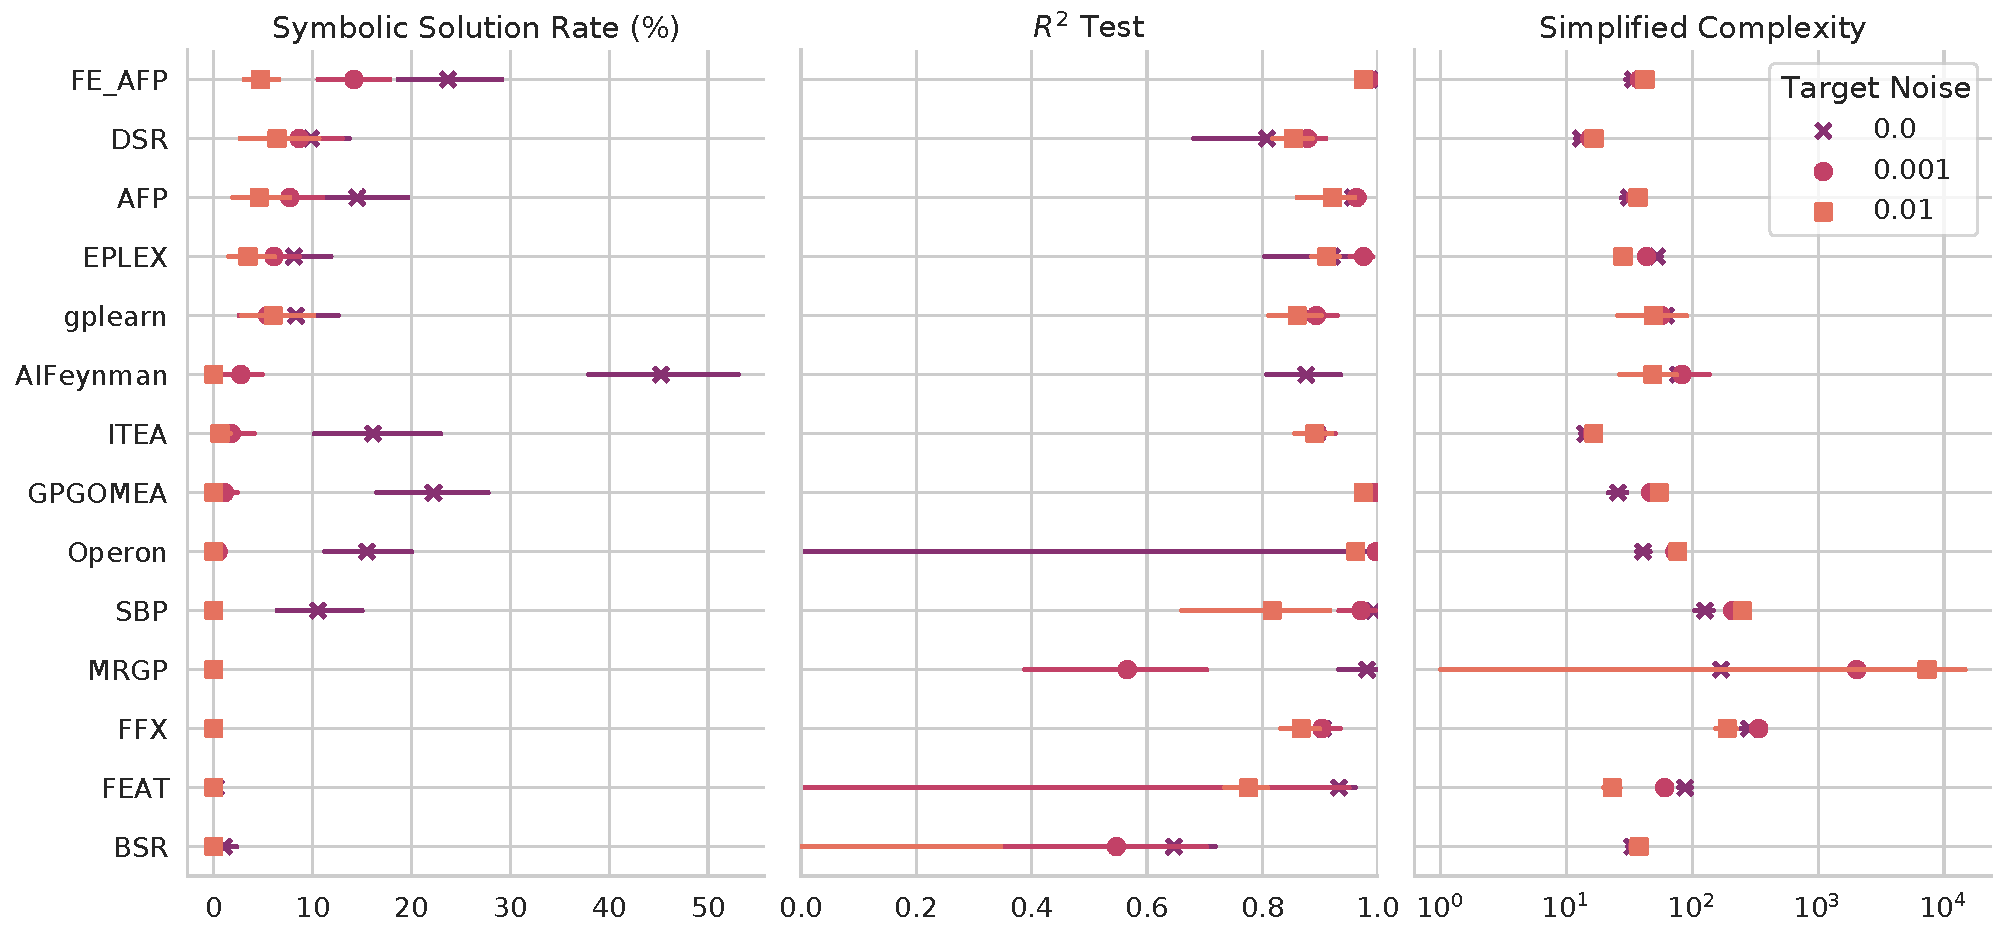
\includegraphics[width=\textwidth]{figs/results_sym_data/pairgrid_symbolic_solution_rate_(pct)_r2_test_simplified_complexity.pdf}
    % \begin{minipage}{0.49\textwidth}
    %     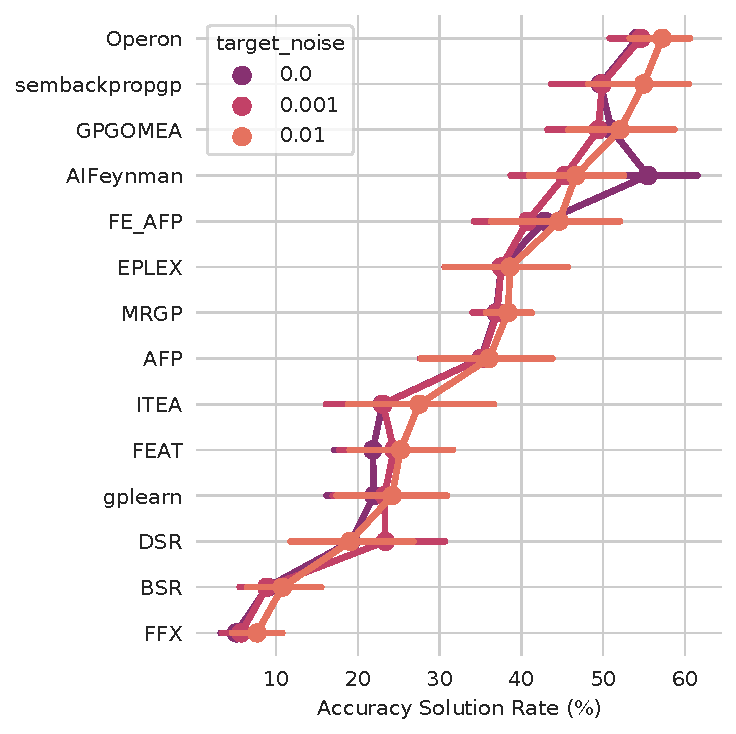
\includegraphics[width=\textwidth]{figs/results_sym_data/cat-pointplot-Accuracy-Solution-Rate-(pct)-by-Algorithm.pdf}
    % \end{minipage}
    % % \hspace{0.01\textwidth}
    % \begin{minipage}{0.49\textwidth}
    %     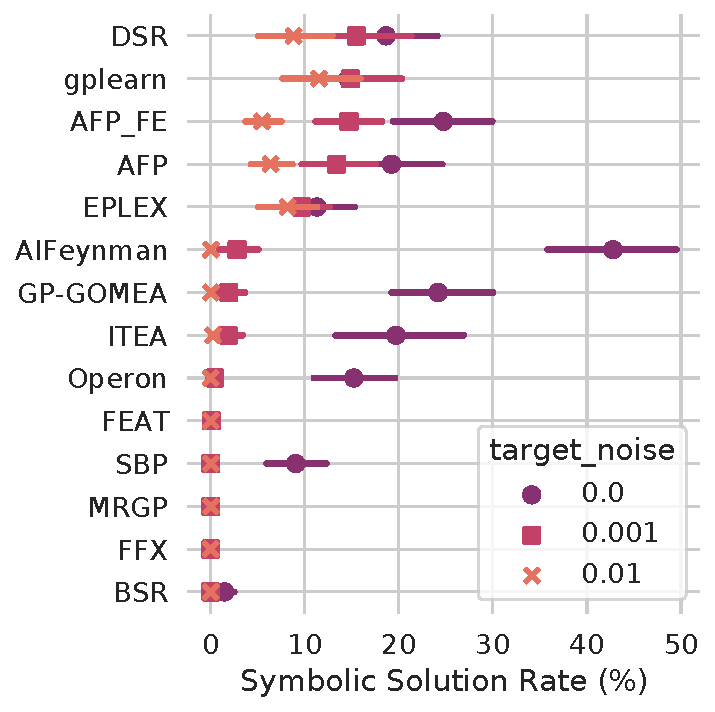
\includegraphics[width=\textwidth]{figs/results_sym_data/cat-pointplot-Symbolic-Solution-Rate-(pct)-by-Algorithm.pdf}
    % \end{minipage}
    \caption{
        Solution rates in terms of perfect accuracy (Left) versus symbolic equivalence (Right) for the Feynman and Strogatz problems. 
        Color indicates level of noise added to the target variable. 
    }
    \label{fig:symbolic_solns}
\end{figure}

% runtime, complexity 
% pareto curves
% Since we are concerned with accuracy as well as simplicity, we take "state-of-the-art" to mean methods that are on the Pareto front of accuracy and simplicity. 
We estimate and visualize the Pareto front for black-box and ground-truth regression in Figure~\ref{fig:pareto}. 

% \begin{wrapfigure}{r}{0.6\textwidth}
\begin{figure}
    \centering
    % \begin{minipage}{0.49\textwidth}
    \includegraphics[width=0.6\textwidth]{figs/results_pmlb_r1/pareto_plot_r2_test_rank_model_size_rank.pdf}
    % \end{minipage}
    % \hspace{0.01\textwidth}
    % \begin{minipage}{0.49\textwidth}
    %     \includegraphics[width=\textwidth]{figs/results_sym_data/pareto_plot_r2_test_rank_model_size_rank.pdf}
    % \end{minipage}
    \caption{
        Pareto plots comparing the rankings of SR methods in terms of model size and $R^2$ score; (left) black-box problems, (right) ground-truth problems.
        Points are the median ranking across datasets, and the bars represent 95\% confidence intervals. 
    } \label{fig:pareto}
\end{figure}
% \end{wrapfigure}

%%%%%%%%%%%%%%%%%%%%%%%%%%%%%%%%%%%%%%%%%%%%%%%%%%%%%%%%%%%%%%%%%%%%%%%%%%%%%%%%
\section{Discussion and Conclusions}
%%%%%%%%%%%%%%%%%%%%%%%%%%%%%%%%%%%%%%%%%%%%%%%%%%%%%%%%%%%%%%%%%%%%%%%%%%%%%%%%
\begin{itemize}
    \item directions for improvement in SR
    \begin{itemize}
        \item running time
        \item tolerance to noise
        \item post-run pruning
    \end{itemize}
    \item improvements to benchmarks
    \begin{itemize}
        \item feature noise
        \item add observations of systems with known dynamics. Caveat: real systems and first principles don't always line up, as in metabolic systems~\cite{yeast} and fluid dynamics \cite{lacavaInferenceCompactNonlinear2016}. 
        \item additional methods: cartesian gp, grammar VAE, etc...
    \end{itemize}
\end{itemize}

\paragraph{Tolerance to noise}


% \section{Submissions to the NeurIPS 2021 Track on Datasets and Benchmarks}

% Please read the instructions below carefully and follow them faithfully.

% \subsection{Style}

% Papers must be prepared according to the
% instructions presented here. Papers may only be up to {\bf nine} pages long,
% including figures. Additional pages \emph{containing only acknowledgments and
% references} are allowed. Papers that exceed the page limit will not be
% reviewed, or in any other way considered for presentation at the conference.

% Authors are required to use the NeurIPS \LaTeX{} style files obtainable at the
% NeurIPS website as indicated below. Please make sure you use the current files
% and not previous versions. Tweaking the style files may be grounds for
% rejection.

% \subsection{Retrieval of style files}

% The style files for the NeurIPS Track on Datasets and Benchmarks and other information are available on the World Wide Web at
% \begin{center}
%   \url{https://urldefense.com/v3/__http://www.neurips.cc/Conferences/2021/CallForDatasetsBenchmarks__;!!GX6Nv3_Pjr8b-17qtCok029Ok438DqXQ!gLfRVZbnI5EEpjSs2SUEUt3REx61nOcbbaUjq8m9DBea3vF6r9tqUapXTgdh$ }
% \end{center}
% The file \verb+neurips_data_2021.pdf+ contains these instructions and illustrates the
% various formatting requirements your submission must satisfy.

% The only supported style file for NeurIPS 2021 is \verb+neurips_data_2021.sty+,
% written for \LaTeXe{}. There are no supported style sheets for Microsoft Word, RTF, or other formats. The \LaTeX{} style file contains three optional arguments: \verb+final+, which
% creates a camera-ready copy, \verb+preprint+, which creates a preprint for
% submission to, e.g., arXiv, and \verb+nonatbib+, which will not load the
% \verb+natbib+ package for you in case of package clash.

% \paragraph{Preprint option}
% If you wish to post a preprint of your work online, e.g., on arXiv, using the
% NeurIPS style, please use the \verb+preprint+ option. This will create a version of your work with the text ``Preprint. Work in progress.''
% in the footer. This version may be distributed as you see fit. Please \textbf{do
%   not} use the \verb+final+ option, which should \textbf{only} be used for
% papers accepted to the NeurIPS Track on Datasets and Benchmarks.

% At submission time, please omit the \verb+final+ and \verb+preprint+
% options. This will add line numbers to aid
% review. Please do \emph{not} refer to these line numbers in your paper as they
% will be removed during generation of camera-ready copies. Note that submissions to the NeurIPS Track on Datasets and Benchmarks are reviewed in a single-blind fashion and therefore not anonymous. This is because datasets can typically not be shared in a non-anonymous way. If you feel strongly that your work should be submitted anonymously, please use the \verb+anonymous+ option. This will create a version of your work with all author names hidden.

% The file \verb+neurips_data_021.tex+ may be used as a ``shell'' for writing your
% paper. All you have to do is replace the author, title, abstract, and text of
% the paper with your own.

% The formatting instructions contained in these style files are summarized in
% Sections \ref{gen_inst}, \ref{headings}, and \ref{others} below.

% \section{General formatting instructions}
% \label{gen_inst}

% The text must be confined within a rectangle 5.5~inches (33~picas) wide and
% 9~inches (54~picas) long. The left margin is 1.5~inch (9~picas).  Use 10~point
% type with a vertical spacing (leading) of 11~points.  Times New Roman is the
% preferred typeface throughout, and will be selected for you by default.
% Paragraphs are separated by \nicefrac{1}{2}~line space (5.5 points), with no
% indentation.

% The paper title should be 17~point, initial caps/lower case, bold, centered
% between two horizontal rules. The top rule should be 4~points thick and the
% bottom rule should be 1~point thick. Allow \nicefrac{1}{4}~inch space above and
% below the title to rules. All pages should start at 1~inch (6~picas) from the
% top of the page.

% Authors' names are set in boldface, and each name is
% centered above the corresponding address. The lead author's name is to be listed
% first (left-most), and the co-authors' names (if different address) are set to
% follow. If there is only one co-author, list both author and co-author side by
% side.

% Please pay special attention to the instructions in Section \ref{others}
% regarding figures, tables, acknowledgments, and references.

% \section{Headings: first level}
% \label{headings}

% All headings should be lower case (except for first word and proper nouns),
% flush left, and bold.

% First-level headings should be in 12-point type.

% \subsection{Headings: second level}

% Second-level headings should be in 10-point type.

% \subsubsection{Headings: third level}

% Third-level headings should be in 10-point type.

% \paragraph{Paragraphs}

% There is also a \verb+\paragraph+ command available, which sets the heading in
% bold, flush left, and inline with the text, with the heading followed by 1\,em
% of space.

% \section{Citations, figures, tables, references}
% \label{others}

% These instructions apply to everyone.

% \subsection{Citations within the text}

% The \verb+natbib+ package will be loaded for you by default.  Citations may be
% author/year or numeric, as long as you maintain internal consistency.  As to the
% format of the references themselves, any style is acceptable as long as it is
% used consistently.

% The documentation for \verb+natbib+ may be found at
% \begin{center}
%   \url{https://urldefense.com/v3/__http://mirrors.ctan.org/macros/latex/contrib/natbib/natnotes.pdf__;!!GX6Nv3_Pjr8b-17qtCok029Ok438DqXQ!gLfRVZbnI5EEpjSs2SUEUt3REx61nOcbbaUjq8m9DBea3vF6r9tqUWshWJ0M$ }
% \end{center}
% Of note is the command \verb+\citet+, which produces citations appropriate for
% use in inline text.  For example,
% \begin{verbatim}
%    \citet{hasselmo} investigated\dots
% \end{verbatim}
% produces
% \begin{quote}
%   Hasselmo, et al.\ (1995) investigated\dots
% \end{quote}

% If you wish to load the \verb+natbib+ package with options, you may add the
% following before loading the \verb+neurips_2021+ package:
% \begin{verbatim}
%    \PassOptionsToPackage{options}{natbib}
% \end{verbatim}

% If \verb+natbib+ clashes with another package you load, you can add the optional
% argument \verb+nonatbib+ when loading the style file:
% \begin{verbatim}
%    \usepackage[nonatbib]{neurips_2021}
% \end{verbatim}

% As submission is double blind, refer to your own published work in the third
% person. That is, use ``In the previous work of Jones et al.\ [4],'' not ``In our
% previous work [4].'' If you cite your other papers that are not widely available
% (e.g., a journal paper under review), use anonymous author names in the
% citation, e.g., an author of the form ``A.\ Anonymous.''

% \subsection{Footnotes}

% Footnotes should be used sparingly.  If you do require a footnote, indicate
% footnotes with a number\footnote{Sample of the first footnote.} in the
% text. Place the footnotes at the bottom of the page on which they appear.
% Precede the footnote with a horizontal rule of 2~inches (12~picas).

% Note that footnotes are properly typeset \emph{after} punctuation
% marks.\footnote{As in this example.}

% \subsection{Figures}

% \begin{figure}
%   \centering
%   \fbox{\rule[-.5cm]{0cm}{4cm} \rule[-.5cm]{4cm}{0cm}}
%   \caption{Sample figure caption.}
% \end{figure}

% All artwork must be neat, clean, and legible. Lines should be dark enough for
% purposes of reproduction. The figure number and caption always appear after the
% figure. Place one line space before the figure caption and one line space after
% the figure. The figure caption should be lower case (except for first word and
% proper nouns); figures are numbered consecutively.

% You may use color figures.  However, it is best for the figure captions and the
% paper body to be legible if the paper is printed in either black/white or in
% color.

% \subsection{Tables}

% All tables must be centered, neat, clean and legible.  The table number and
% title always appear before the table.  See Table~\ref{sample-table}.

% Place one line space before the table title, one line space after the
% table title, and one line space after the table. The table title must
% be lower case (except for first word and proper nouns); tables are
% numbered consecutively.

% Note that publication-quality tables \emph{do not contain vertical rules.} We
% strongly suggest the use of the \verb+booktabs+ package, which allows for
% typesetting high-quality, professional tables:
% \begin{center}
%   \url{https://urldefense.com/v3/__https://www.ctan.org/pkg/booktabs__;!!GX6Nv3_Pjr8b-17qtCok029Ok438DqXQ!gLfRVZbnI5EEpjSs2SUEUt3REx61nOcbbaUjq8m9DBea3vF6r9tqUazm7Esl$ }
% \end{center}
% This package was used to typeset Table~\ref{sample-table}.

% \begin{table}
%   \caption{Sample table title}
%   \label{sample-table}
%   \centering
%   \begin{tabular}{lll}
%     \toprule
%     \multicolumn{2}{c}{Part}                   \\
%     \cmidrule(r){1-2}
%     Name     & Description     & Size ($\mu$m) \\
%     \midrule
%     Dendrite & Input terminal  & $\sim$100     \\
%     Axon     & Output terminal & $\sim$10      \\
%     Soma     & Cell body       & up to $10^6$  \\
%     \bottomrule
%   \end{tabular}
% \end{table}

% \section{Final instructions}

% Do not change any aspects of the formatting parameters in the style files.  In
% particular, do not modify the width or length of the rectangle the text should
% fit into, and do not change font sizes (except perhaps in the
% \textbf{References} section; see below). Please note that pages should be
% numbered.

% \section{Preparing PDF files}

% Please prepare submission files with paper size ``US Letter,'' and not, for
% example, ``A4.''

% Fonts were the main cause of problems in the past years. Your PDF file must only
% contain Type 1 or Embedded TrueType fonts. Here are a few instructions to
% achieve this.

% \begin{itemize}

% \item You should directly generate PDF files using \verb+pdflatex+.

% \item You can check which fonts a PDF files uses.  In Acrobat Reader, select the
%   menu Files$>$Document Properties$>$Fonts and select Show All Fonts. You can
%   also use the program \verb+pdffonts+ which comes with \verb+xpdf+ and is
%   available out-of-the-box on most Linux machines.

% \item The IEEE has recommendations for generating PDF files whose fonts are also
%   acceptable for NeurIPS. Please see
%   \url{https://urldefense.com/v3/__http://www.emfield.org/icuwb2010/downloads/IEEE-PDF-SpecV32.pdf__;!!GX6Nv3_Pjr8b-17qtCok029Ok438DqXQ!gLfRVZbnI5EEpjSs2SUEUt3REx61nOcbbaUjq8m9DBea3vF6r9tqUdJHXlva$ }

% \item \verb+xfig+ "patterned" shapes are implemented with bitmap fonts.  Use
%   "solid" shapes instead.

% \item The \verb+\bbold+ package almost always uses bitmap fonts.  You should use
%   the equivalent AMS Fonts:
% \begin{verbatim}
%    \usepackage{amsfonts}
% \end{verbatim}
% followed by, e.g., \verb+\mathbb{R}+, \verb+\mathbb{N}+, or \verb+\mathbb{C}+
% for $\mathbb{R}$, $\mathbb{N}$ or $\mathbb{C}$.  You can also use the following
% workaround for reals, natural and complex:
% \begin{verbatim}
%    \newcommand{\RR}{I\!\!R} %real numbers
%    \newcommand{\Nat}{I\!\!N} %natural numbers
%    \newcommand{\CC}{I\!\!\!\!C} %complex numbers
% \end{verbatim}
% Note that \verb+amsfonts+ is automatically loaded by the \verb+amssymb+ package.

% \end{itemize}

% If your file contains type 3 fonts or non embedded TrueType fonts, we will ask
% you to fix it.

% \subsection{Margins in \LaTeX{}}

% Most of the margin problems come from figures positioned by hand using
% \verb+\special+ or other commands. We suggest using the command
% \verb+\includegraphics+ from the \verb+graphicx+ package. Always specify the
% figure width as a multiple of the line width as in the example below:
% \begin{verbatim}
%    \usepackage[pdftex]{graphicx} ...
%    \includegraphics[width=0.8\linewidth]{myfile.pdf}
% \end{verbatim}
% See Section 4.4 in the graphics bundle documentation
% (\url{https://urldefense.com/v3/__http://mirrors.ctan.org/macros/latex/required/graphics/grfguide.pdf__;!!GX6Nv3_Pjr8b-17qtCok029Ok438DqXQ!gLfRVZbnI5EEpjSs2SUEUt3REx61nOcbbaUjq8m9DBea3vF6r9tqUZ5WNA5f$ })

% A number of width problems arise when \LaTeX{} cannot properly hyphenate a
% line. Please give LaTeX hyphenation hints using the \verb+\-+ command when
% necessary.

\begin{ack}
% Use unnumbered first level headings for the acknowledgments. All acknowledgments
% go at the end of the paper before the list of references. Moreover, you are required to declare
% funding (financial activities supporting the submitted work) and competing interests (related financial activities outside the submitted work).
% More information about this disclosure can be found at: \url{https://urldefense.com/v3/__https://neurips.cc/Conferences/2021/PaperInformation/FundingDisclosure__;!!GX6Nv3_Pjr8b-17qtCok029Ok438DqXQ!gLfRVZbnI5EEpjSs2SUEUt3REx61nOcbbaUjq8m9DBea3vF6r9tqUTr1seQz$ }.

% Do {\bf not} include this section in the anonymized submission, only in the final paper. You can use the \texttt{ack} environment provided in the style file to autmoatically hide this section in the anonymized submission.
    William La~Cava was supported by NIH/NLM grant K99LM012926 and would like to thank Curt Calafut and the Penn Medicine Academic Computing Services (PMACS) for supporting the computational load, and members of the Epistasis Lab for their patience.   
    Computational support was provided by the Penn 
    Ying Jin would like to thank Doctor Jian Guo for hosting an internship for the project and Professor Jian Kang for helpful and inspiring guidances in Bayesian statistics.
    Authors declare no competing interests. 
\end{ack}

% \section*{References}

% References follow the acknowledgments. Use unnumbered first-level heading for
% the references. Any choice of citation style is acceptable as long as you are
% consistent. It is permissible to reduce the font size to \verb+small+ (9 point)
% when listing the references.
% Note that the Reference section does not count towards the page limit.
\medskip

{
\small

\bibliographystyle{plainnat}
\bibliography{SymbolicRegression}
}

%%%%%%%%%%%%%%%%%%%%%%%%%%%%%%%%%%%%%%%%%%%%%%%%%%%%%%%%%%%%
\section*{Checklist}

%%% BEGIN INSTRUCTIONS %%%
The checklist follows the references.  Please
read the checklist guidelines carefully for information on how to answer these
questions.  For each question, change the default \answerTODO{} to \answerYes{},
\answerNo{}, or \answerNA{}.  You are strongly encouraged to include a {\bf
justification to your answer}, either by referencing the appropriate section of
your paper or providing a brief inline description.  For example:
\begin{itemize}
  \item Did you include the license to the code and datasets? \answerYes{See Section~\ref{gen_inst}.}
  \item Did you include the license to the code and datasets? \answerNo{The code and the data are proprietary.}
  \item Did you include the license to the code and datasets? \answerNA{}
\end{itemize}
Please do not modify the questions and only use the provided macros for your
answers.  Note that the Checklist section does not count towards the page
limit.  In your paper, please delete this instructions block and only keep the
Checklist section heading above along with the questions/answers below.
%%% END INSTRUCTIONS %%%

\begin{enumerate}

\item For all authors...
\begin{enumerate}
  \item Do the main claims made in the abstract and introduction accurately reflect the paper's contributions and scope?
    \answerTODO{}
  \item Did you describe the limitations of your work?
    \answerTODO{}
  \item Did you discuss any potential negative societal impacts of your work?
    \answerTODO{}
  \item Have you read the ethics review guidelines and ensured that your paper conforms to them?
    \answerTODO{}
\end{enumerate}

\item If you are including theoretical results...
\begin{enumerate}
  \item Did you state the full set of assumptions of all theoretical results?
    \answerTODO{}
	\item Did you include complete proofs of all theoretical results?
    \answerTODO{}
\end{enumerate}

\item If you ran experiments (e.g. for benchmarks)...
\begin{enumerate}
  \item Did you include the code, data, and instructions needed to reproduce the main experimental results (either in the supplemental material or as a URL)?
    \answerTODO{}
  \item Did you specify all the training details (e.g., data splits, hyperparameters, how they were chosen)?
    \answerTODO{}
	\item Did you report error bars (e.g., with respect to the random seed after running experiments multiple times)?
    \answerTODO{}
	\item Did you include the total amount of compute and the type of resources used (e.g., type of GPUs, internal cluster, or cloud provider)?
    \answerTODO{}
\end{enumerate}

\item If you are using existing assets (e.g., code, data, models) or curating/releasing new assets...
\begin{enumerate}
  \item If your work uses existing assets, did you cite the creators?
    \answerTODO{}
  \item Did you mention the license of the assets?
    \answerTODO{}
  \item Did you include any new assets either in the supplemental material or as a URL?
    \answerTODO{}
  \item Did you discuss whether and how consent was obtained from people whose data you're using/curating?
    \answerTODO{}
  \item Did you discuss whether the data you are using/curating contains personally identifiable information or offensive content?
    \answerTODO{}
\end{enumerate}

\item If you used crowdsourcing or conducted research with human subjects...
\begin{enumerate}
  \item Did you include the full text of instructions given to participants and screenshots, if applicable?
    \answerTODO{}
  \item Did you describe any potential participant risks, with links to Institutional Review Board (IRB) approvals, if applicable?
    \answerTODO{}
  \item Did you include the estimated hourly wage paid to participants and the total amount spent on participant compensation?
    \answerTODO{}
\end{enumerate}

\end{enumerate}

%%%%%%%%%%%%%%%%%%%%%%%%%%%%%%%%%%%%%%%%%%%%%%%%%%%%%%%%%%%%

\appendix

\section{Appendix}


Include extra information in the appendix. This section will often be part of the supplemental material. Please see the call on the NeurIPS website for links to additional guides on dataset publication.

\begin{enumerate}

% \item Submission introducing new datasets must include the following in the supplementary materials:
% \begin{enumerate}
  % \item Dataset documentation and intended uses. Recommended documentation frameworks include datasheets for datasets, dataset nutrition labels, data statements for NLP, and accountability frameworks.
  % \item URL to website/platform where the dataset/benchmark can be viewed and downloaded by the reviewers.
  % \item Author statement that they bear all responsibility in case of violation of rights, etc., and confirmation of the data license.
  % \item Hosting, licensing, and maintenance plan. The choice of hosting platform is yours, as long as you ensure access to the data (possibly through a curated interface) and will provide the necessary maintenance.
% \end{enumerate}

\item To ensure accessibility, the supplementary materials for datasets must include the following:
\begin{enumerate}
  % \item Links to access the dataset and its metadata. This can be hidden upon submission if the dataset is not yet publicly available but must be added in the camera-ready version. In select cases, e.g when the data can only be released at a later date, this can be added afterward. Simulation environments should link to (open source) code repositories.
  % \item The dataset itself should ideally use an open and widely used data format. Provide a detailed explanation on how the dataset can be read. For simulation environments, use existing frameworks or explain how they can be used.
  % \item Long-term preservation: It must be clear that the dataset will be available for a long time, either by uploading to a data repository or by explaining how the authors themselves will ensure this.
  % \item Explicit license: Authors must choose a license, ideally a CC license for datasets, or an open source license for code (e.g. RL environments).
  % \item Add structured metadata to a dataset's meta-data page using Web standards (like schema.org and DCAT): This allows it to be discovered and organized by anyone. If you use an existing data repository, this is often done automatically.
  \item Highly recommended: a persistent dereferenceable identifier (e.g. a DOI minted by a data repository or a prefix on identifiers.org) for datasets, or a code repository (e.g. GitHub, GitLab,...) for code. If this is not possible or useful, please explain why.
\end{enumerate}

\item For benchmarks, the supplementary materials must ensure that all results are easily reproducible. Where possible, use a reproducibility framework such as the ML reproducibility checklist, or otherwise guarantee that all results can be easily reproduced, i.e. all necessary datasets, code, and evaluation procedures must be accessible and documented.

\item For papers introducing best practices in creating or curating datasets and benchmarks, the above supplementary materials are not required.
\end{enumerate}

Please refer to \url{https://github.com/EpistasisLab/srbench/} for the most up-to-date guide to running the benchmark study. 

\subsection{Running the Benchmark}

\subsection{Contributing a Method}
A living version of the method contribution instructions are described in the \href{https://github.com/EpistasisLab/srbench/blob/master/CONTRIBUTING.md}{Contribution Guide}.
To illustrate the simplicity of contributing a method, Figure~\ref{fig:ex_code} shows the script submitted for Bayesian Symbolic Regression~\cite{jinBayesianSymbolicRegression2020}. 
In addition to the code snippet, authors may either add their code package to the conda/pip environment, or provide an install script.
When a pull request is issued by a contributor, new methods and installs are automatically tested on a minimal version of the benchmark.  

\begin{figure}
	\DeclareTCBListing{mintedbox}{O{}m!O{}}{%
  breakable=true,
  listing engine=minted,
  listing only,
  minted language=#2,
  minted style=default,
  minted options={%
    linenos,
    gobble=0,
    breaklines=true,
    breakafter=,,
    fontsize=\footnotesize,
    numbersep=8pt,
    #1},
  boxsep=0pt,
  left skip=0pt,
  right skip=0pt,
  left=25pt,
  right=0pt,
  top=3pt,
  bottom=3pt,
  arc=5pt,
  leftrule=0pt,
  rightrule=0pt,
  bottomrule=2pt,
  toprule=2pt,
  colback=bg,
  colframe=orange!70,
  enhanced,
  overlay={%
    \begin{tcbclipinterior}
    \fill[orange!20!white] (frame.south west) rectangle ([xshift=20pt]frame.north west);
    \end{tcbclipinterior}},
  #3}
\begin{mintedbox}{python}
# method: Bayesian Symbolic Regression
# contributor: Ying Jin
# source: https://github.com/ying531/MCMC-SymReg
from bsr.bsr_class import BSR

hyper_params = []
for val, itrNum in zip([100,500,1000],[5000,1000,500]):
    for treeNum in [3,6]:
        hyper_params.append(
                    {'treeNum': [treeNum], 
                     'itrNum': [itrNum], 
                     'val': [val],
                    })
# default estimator
est = BSR(val=100, itrNum=5000, treeNum=3, alpha1=0.4, alpha2=0.4, 
          beta=-1, disp=False, max_time=2*60*60)

def complexity(est):
"""returns final model complexity"""
    return est.complexity()

def model(est):
"""returns final model as string"""
    return est.model()
\end{mintedbox}


    \caption{
        An example code contribution, defining the estimator, its hyperparameters, and functions to return the complexity and symbolic model.
    }\label{fig:ex_code} 
\end{figure}

\subsection{Additional Background and Motivation}

Eureqa is a closed-source commercial software that was acquired by DataRobot in 2017\footnote{\url{https://www.datarobot.com/nutonian/}}. 
Due to its proprietary nature and incorporation into the DataRobot platform, it is impossible to benchmark its performance while controlling for important experimental variables such as computational effort. 
However, the algorithmic aspects of Eureqa are described in literature and summarized here. 
First is its use of directed acyclic graphs for representing equations in lieu of trees, which resulted in more space-efficient encodings without a significant difference in performance~\cite{schmidtComparisonTreeGraph2007}. 
The most significant improvement over traditional tournament-based selection is Eureqa's use of age-fitness Pareto optimization (AFP), a method in which random restarts are incorporated each generation as new offspring, and are protected from competing with older, more fit equations by including age as an objective to be minimized~\cite{schmidtAgefitnessParetoOptimization2011}. 
Eureqa also includes the co-evolution of fitness predictors, in which fitness assignment is sped up by optimizing a second population of training sample indices that best distinguish between equations in the population~\cite{schmidtCoevolutionFitnessPredictors2008}.
It is also possible that Eureqa no longer uses any of these reported algorithms for SR, due to its closed-source nature.
In that light, it is not clear what fundamental insight is gained when comparing to the software itself, other than a head-to-head comparison, since methodological insights cannot be extracted.

Moreover, Eureqa's multi-objective optimization strategy (age-fitness pareto optimization~\cite{schmidtAgefitnessParetoOptimization2011}) has been outperformed by a number of other optimization methods (e.g.,~\cite{lacavaEpsilonLexicaseSelectionRegression2016c,liskowskiDiscoverySearchObjectives2017}), some of which are included in our study.
Many other lines of research have pointed in promising directions, including hybridizations of GP with local search for constant optimization~\cite{topchyFasterGeneticProgramming2001,kommendaParameterIdentificationSymbolic2019} or structural tuning~\cite{lacavaInferenceCompactNonlinear2016}; the increasing use of \textit{semantic methods} for guiding variation~\cite{moraglioGeometricSemanticGenetic2012a,virgolinLinearScalingSemantic2019} and selection~\cite{azadKrzysztofKrawiecBehavioral2017,lacavaProbabilisticMultiobjectiveAnalysis2019,arnaldoMultipleRegressionGenetic2014a}; and alternative representations of equations~\cite{defrancaInteractionTransformationEvolutionaryAlgorithm2020,mcconaghyFFXFastScalable2011}.
The term \textit{semantic methods} refers to evolutionary strategies that leverage the full behavior (i.e. semantics) of the model, and potentially its subcomponents, to drive search, rather than relying on aggregate, scalar fitness values~\cite{vanneschiSurveySemanticMethods2014}.




\subsection{Additional Dataset Information}

All datasets, including metadata, are available from \href{https://epistasislab.github.io/pmlb/}{PMLB}. 
Each dataset is stored using Git Large File Storage and PMLB is planned for long-term maintenance.
PMLB is available under an MIT license, and is described in detail in~\citet{romanoPMLBV1Open2021}. 
The authors bear all responsibility in case of violation of rights.

\paragraph{Ethical Considerations and Intended Uses}
PMLB is intended to be used as a framework for benchmarking ML and SR algorithms and as a resource for investigating the structure of datasets. 
This paper does not contribute new datasets, but rather collates and standardizes datasets that were already publicly available.
In that regard, we do not foresee it as creating additional ethical issues around their use. 
However, it is worth noting that PMLB contains well-known, real-world datasets from UCI and OpenML for which ethical considerations are important, such as the \href{https://github.com/EpistasisLab/pmlb/blob/master/datasets/1089_USCrime/metadata.yaml}{USCrime} dataset. 
Whereas we would view the risk of harm arising specifically from this dataset to be low (the data is from 1960), it is exemplary of a task for which algorithmic decision making could exacerbate existing biases in the criminal justice system.  
As such it is used as a benchmark in a number of papers in the ML fairness literature (e.g.~\cite{kearnsPreventingFairnessGerrymandering2018}). 


\paragraph{Feynman datasets}
The Feynman benchmarks were sourced from the \href{https://space.mit.edu/home/tegmark/aifeynman.html}{Feynman Symbolic Regression Database}. 
We standardized the Feynman and Bonus equations to PMLB format and included metadata detailing the model form and the units for each variable. 
We used the version of the equations that were not simplified by dimensional analysis. 
\citet{udrescuAIFeynmanPhysicsInspired2020} describe each dataset as containing $10^5$ rows, but each actually contains $10^6$. 
Given this discrepancy and after noting that subsampling did not significantly change the correlation structure of any of the problems, each dataset was downsampled from 1 million samples to 100,000 to lower the computational burden.
We also observed that Eqn. II.11.17 was missing from the database. 
Finally, we excluded three datasets from our analysis that contained $\arcsin$ and $\arccos$ functions, as these were not implemented in the majority of SR algorithms we tested.

\paragraph{Strogatz datasets}
The Strogatz datasets were sourced from the \href{https://github.com/lacava/ode-strogatz}{ODE-Strogatz repository}~\cite{lacavaInferenceCompactNonlinear2016}.
Each dataset is one state of a 2-state system of first-order, ordinary differential equations (ODEs). 
The goal of each problem is to predict rate of change of the state given the current two states on which it depends. 
Each represents natural processes that exhibit chaos and non-linear dynamics.
The problems were originally adapted from~\cite{strogatzNonlinearDynamicsChaos2014} by~\citet{schmidtMachineScienceAutomated2011}.   
In order to simulate their behavior, initial conditions were chosen within stable basins of attraction.
Each system was simulated using Simulink, and the simulation code is available in the repository above.
The equations for each of these datasets are shown in Table~\ref{tbl:strogatz}.

\begin{table}[htb]
\scriptsize
\centering
\renewcommand{\arraystretch}{1.2}\addtolength{\tabcolsep}{.5pt}
\caption{The Strogatz ODE problems. 
         } \label{tbl:strogatz}
% \rowcolors{3}{white}{lightgray}
\begin{tabular}{ll} %L{0.12\textwidth} L{0.25\textwidth} L{0.25\textwidth} L{0.25\textwidth} } \toprule 
 Name & Target \\ \toprule 
Bacterial Respiration                   & $\dot{x} = 20 - x - \frac{x \cdot y}{1+0.5 \cdot x^2}$ \\	
                                        & $ \dot{y} = 10 - \frac{x \cdot y}{1+0.5 \cdot x^2}$	\\ 
\midrule
Bar Magnets                             & $\dot{\theta} = 0.5 \cdot \sin (\theta - \phi) - \sin (\theta)$	\\
                                        & $ \dot{\phi} = 0.5 \cdot \sin (\phi - \theta) - \sin (\phi)$ \\ 
\midrule
Glider                                  & $\dot{v} = - 0.05 \cdot  v^2 - sin (\theta)$	\\
                                        & $ \dot{\theta} = v - \cos (\theta)/v$	\\ 
\midrule
Lotka-Volterra interspecies dynamics    & $\dot{x} = 3  \cdot x - 2  \cdot x \cdot y - x^2$	\\
                                        & $ \dot{y} = 2 \cdot y - x \cdot y - y^2$	\\ 
\midrule
Predator Prey                           & $\dot{x} = x  \cdot \left( 4 - x - \frac{y}{1+x} \right)$	\\
                                        & $\dot{y} = y \cdot \left( \frac{x}{1+x} - 0.075 \cdot y \right)$	\\ 
\midrule
Shear Flow                              & $\dot{\theta} = \cot (\phi) \cdot cos(\theta)$	\\
                                        & $ \dot{\phi} = \left(\cos ^2 (\phi) + 0.1 \cdot  \sin^2 (\phi)\right) \cdot sin(\theta)$	\\ 
\midrule
van der Pol oscillator                  & $\dot{x} = 10 \cdot  \left(y - \frac{1}{3} \cdot (x^3-x) \right)$	\\
                                        & $ \dot{y} = -\frac{1}{10} \cdot x$ \\
\bottomrule
\end{tabular}
\end{table}


\subsection{Additional Experiment Details}

%% LPC


%% dealing with fails

%% Hyperparameters of each method
\begin{table}
    \footnotesize
    \centering

    \caption{
        ML methods and the hyperparameter spaces used in tuning.
    }
	\label{tbl:ml_methods}
    \rowcolors{2}{gray!25}{white}
    \begin{tabular}{l p{37em}}
\toprule
          Method &                                                                                                                                                          Hyperparameters \\
\midrule
        AdaBoost &                                                                                               \{'learning\_rate': (0.01, 0.1, 1.0, 10.0), 'n\_estimators': (10, 100, 1000)\} \\
     KernelRidge &                                                           \{'kernel': ('linear', 'poly', 'rbf', 'sigmoid'), 'alpha': (0.0001, 0.01, 0.1, 1), 'gamma': (0.01, 0.1, 1, 10)\} \\
       LassoLars &                                                                                                                                 \{'alpha': (0.0001, 0.001, 0.01, 0.1, 1)\} \\
            LGBM & \{'n\_estimators': (10, 50, 100, 250, 500, 1000), 'learning\_rate': (0.0001, 0.01, 0.05, 0.1, 0.2), 'subsample': (0.5, 0.75, 1), 'boosting\_type': ('gbdt', 'dart', 'goss')\} \\
LinearRegression &                                                                                                                                               \{'fit\_intercept': (True,)\} \\
             MLP &                                \{'activation': ('logistic', 'tanh', 'relu'), 'solver': ('lbfgs', 'adam', 'sgd'), 'learning\_rate': ('constant', 'invscaling', 'adaptive')\} \\
    RandomForest &                                                  \{'n\_estimators': (10, 100, 1000), 'min\_weight\_fraction\_leaf': (0.0, 0.25, 0.5), 'max\_features': ('sqrt', 'log2', None)\} \\
             SGD &                                                                                               \{'alpha': (1e-06, 0.0001, 0.01, 1), 'penalty': ('l2', 'l1', 'elasticnet')\} \\
             XGB &          \{'n\_estimators': (10, 50, 100, 250, 500, 1000), 'learning\_rate': (0.0001, 0.01, 0.05, 0.1, 0.2), 'gamma': (0, 0.1, 0.2, 0.3, 0.4), 'subsample': (0.5, 0.75, 1)\} \\
\bottomrule
\end{tabular}

    
\end{table}

\begin{table}
    \footnotesize
    \centering
    \caption{
        Part 1: SR methods and the hyperparameter spaces used in tuning on the black-box regression problems.
    }
	\label{tbl:sr_methods1}
    \begin{tabular}{l p{37em}}
\toprule
   Method &                                                                                                      Hyperparameters \\
\midrule
\midrule
      AFP &               \{'popsize': 100, 'g': 2500, 'op\_list': ['n', 'v', '+', '-', '*', '/', 'exp', 'log', '2', '3', 'sqrt']\} \\
          & \{'popsize': 100, 'g': 2500, 'op\_list': ['n', 'v', '+', '-', '*', '/', 'exp', 'log', '2', '3', 'sqrt', 'sin', 'cos']\} \\
          &                \{'popsize': 500, 'g': 500, 'op\_list': ['n', 'v', '+', '-', '*', '/', 'exp', 'log', '2', '3', 'sqrt']\} \\
          &  \{'popsize': 500, 'g': 500, 'op\_list': ['n', 'v', '+', '-', '*', '/', 'exp', 'log', '2', '3', 'sqrt', 'sin', 'cos']\} \\
          &               \{'popsize': 1000, 'g': 250, 'op\_list': ['n', 'v', '+', '-', '*', '/', 'exp', 'log', '2', '3', 'sqrt']\} \\
          & \{'popsize': 1000, 'g': 250, 'op\_list': ['n', 'v', '+', '-', '*', '/', 'exp', 'log', '2', '3', 'sqrt', 'sin', 'cos']\} \\
\midrule
AIFeynman &                                                                               \{'BF\_try\_time': 60, 'NN\_epochs': 4000\} \\
          &                                                                               \{'BF\_try\_time': 60, 'NN\_epochs': 4000\} \\
          &                                                                               \{'BF\_try\_time': 60, 'NN\_epochs': 4000\} \\
          &                                                                               \{'BF\_try\_time': 600, 'NN\_epochs': 400\} \\
          &                                                                               \{'BF\_try\_time': 600, 'NN\_epochs': 400\} \\
          &                                                                               \{'BF\_try\_time': 600, 'NN\_epochs': 400\} \\
\midrule
      BSR &                                                                           \{'treeNum': 6, 'itrNum': 500, 'val': 1000\} \\
          &                                                                           \{'treeNum': 6, 'itrNum': 1000, 'val': 500\} \\
          &                                                                           \{'treeNum': 3, 'itrNum': 500, 'val': 1000\} \\
          &                                                                           \{'treeNum': 6, 'itrNum': 5000, 'val': 100\} \\
          &                                                                           \{'treeNum': 3, 'itrNum': 5000, 'val': 100\} \\
          &                                                                           \{'treeNum': 3, 'itrNum': 1000, 'val': 500\} \\
\midrule
      DSR &                                                      \{'batch\_size': array([    10,    100,   1000,  10000, 100000])\} \\
\midrule
    EPLEX &               \{'popsize': 1000, 'g': 250, 'op\_list': ['n', 'v', '+', '-', '*', '/', 'exp', 'log', '2', '3', 'sqrt']\} \\
          &                \{'popsize': 500, 'g': 500, 'op\_list': ['n', 'v', '+', '-', '*', '/', 'exp', 'log', '2', '3', 'sqrt']\} \\
          & \{'popsize': 1000, 'g': 250, 'op\_list': ['n', 'v', '+', '-', '*', '/', 'sin', 'cos', 'exp', 'log', '2', '3', 'sqrt']\} \\
          &               \{'popsize': 100, 'g': 2500, 'op\_list': ['n', 'v', '+', '-', '*', '/', 'exp', 'log', '2', '3', 'sqrt']\} \\
          & \{'popsize': 100, 'g': 2500, 'op\_list': ['n', 'v', '+', '-', '*', '/', 'sin', 'cos', 'exp', 'log', '2', '3', 'sqrt']\} \\
          &  \{'popsize': 500, 'g': 500, 'op\_list': ['n', 'v', '+', '-', '*', '/', 'sin', 'cos', 'exp', 'log', '2', '3', 'sqrt']\} \\
\midrule
     FEAT &                                                                           \{'pop\_size': 100, 'gens': 2500, 'lr': 0.1\} \\
          &                                                                           \{'pop\_size': 100, 'gens': 2500, 'lr': 0.3\} \\
          &                                                                            \{'pop\_size': 500, 'gens': 500, 'lr': 0.1\} \\
          &                                                                            \{'pop\_size': 500, 'gens': 500, 'lr': 0.3\} \\
          &                                                                           \{'pop\_size': 1000, 'gens': 250, 'lr': 0.1\} \\
          &                                                                           \{'pop\_size': 1000, 'gens': 250, 'lr': 0.3\} \\
\midrule
   FE\_AFP & \{'popsize': 1000, 'g': 250, 'op\_list': ['n', 'v', '+', '-', '*', '/', 'sin', 'cos', 'exp', 'log', '2', '3', 'sqrt']\} \\
          &                \{'popsize': 500, 'g': 500, 'op\_list': ['n', 'v', '+', '-', '*', '/', 'exp', 'log', '2', '3', 'sqrt']\} \\
          &               \{'popsize': 1000, 'g': 250, 'op\_list': ['n', 'v', '+', '-', '*', '/', 'exp', 'log', '2', '3', 'sqrt']\} \\
          &               \{'popsize': 100, 'g': 2500, 'op\_list': ['n', 'v', '+', '-', '*', '/', 'exp', 'log', '2', '3', 'sqrt']\} \\
          & \{'popsize': 100, 'g': 2500, 'op\_list': ['n', 'v', '+', '-', '*', '/', 'sin', 'cos', 'exp', 'log', '2', '3', 'sqrt']\} \\
          &  \{'popsize': 500, 'g': 500, 'op\_list': ['n', 'v', '+', '-', '*', '/', 'sin', 'cos', 'exp', 'log', '2', '3', 'sqrt']\} \\
\bottomrule
\end{tabular}
\end{table}

\begin{table}
    \scriptsize

    \centering

    \caption{
        Part 2: SR methods and the hyperparameter spaces used in tuning on the black-box regression problems.
    }
	\label{tbl:sr_methods2}
    \begin{tabular}{l p{37em}}
\toprule
       Method &                                                                                                                                                                                                                                                                                Hyperparameters \\
\midrule
\midrule
      GPGOMEA &                                                                                                                                                                        \{'initmaxtreeheight': (4,), 'functions': ('+\_-\_*\_p/\_plog\_sqrt\_sin\_cos',), 'popsize': (1000,), 'linearscaling': (True,)\} \\
              &                                                                                                                                                                        \{'initmaxtreeheight': (6,), 'functions': ('+\_-\_*\_p/\_plog\_sqrt\_sin\_cos',), 'popsize': (1000,), 'linearscaling': (True,)\} \\
              &                                                                                                                                                                                          \{'initmaxtreeheight': (4,), 'functions': ('+\_-\_*\_p/',), 'popsize': (1000,), 'linearscaling': (True,)\} \\
              &                                                                                                                                                                                          \{'initmaxtreeheight': (6,), 'functions': ('+\_-\_*\_p/',), 'popsize': (1000,), 'linearscaling': (True,)\} \\
              &                                                                                                                                                                       \{'initmaxtreeheight': (4,), 'functions': ('+\_-\_*\_p/\_plog\_sqrt\_sin\_cos',), 'popsize': (1000,), 'linearscaling': (False,)\} \\
              &                                                                                                                                                                       \{'initmaxtreeheight': (6,), 'functions': ('+\_-\_*\_p/\_plog\_sqrt\_sin\_cos',), 'popsize': (1000,), 'linearscaling': (False,)\} \\
\midrule
         ITEA &                                                                                                                                                                             \{'exponents': ((-5, 5),), 'termlimit': ((2, 15),), 'transfunctions': ('[Id, Tanh, Sin, Cos, Log, Exp, SqrtAbs]',)\} \\
              &                                                                                                                                                                              \{'exponents': ((-5, 5),), 'termlimit': ((2, 5),), 'transfunctions': ('[Id, Tanh, Sin, Cos, Log, Exp, SqrtAbs]',)\} \\
              &                                                                                                                                                                                                           \{'exponents': ((-5, 5),), 'termlimit': ((2, 15),), 'transfunctions': ('[Id, Sin]',)\} \\
              &                                                                                                                                                                                                            \{'exponents': ((0, 5),), 'termlimit': ((2, 15),), 'transfunctions': ('[Id, Sin]',)\} \\
              &                                                                                                                                                                                                             \{'exponents': ((0, 5),), 'termlimit': ((2, 5),), 'transfunctions': ('[Id, Sin]',)\} \\
              &                                                                                                                                                                              \{'exponents': ((0, 5),), 'termlimit': ((2, 15),), 'transfunctions': ('[Id, Tanh, Sin, Cos, Log, Exp, SqrtAbs]',)\} \\
\midrule
         MRGP &                                                                                                                                                                                                                                    \{'popsize': 1000, 'g': 250, 'rt\_cross': 0.8, 'rt\_mut': 0.2\} \\
              &                                                                                                                                                                                                                                    \{'popsize': 100, 'g': 2500, 'rt\_cross': 0.2, 'rt\_mut': 0.8\} \\
              &                                                                                                                                                                                                                                    \{'popsize': 100, 'g': 2500, 'rt\_cross': 0.8, 'rt\_mut': 0.2\} \\
              &                                                                                                                                                                                                                                     \{'popsize': 500, 'g': 500, 'rt\_cross': 0.2, 'rt\_mut': 0.8\} \\
              &                                                                                                                                                                                                                                     \{'popsize': 500, 'g': 500, 'rt\_cross': 0.8, 'rt\_mut': 0.2\} \\
              &                                                                                                                                                                                                                                    \{'popsize': 1000, 'g': 250, 'rt\_cross': 0.2, 'rt\_mut': 0.8\} \\
\midrule
       Operon &                  \{'population\_size': (500,), 'pool\_size': (500,), 'max\_length': (50,), 'allowed\_symbols': ('add,mul,aq,constant,variable',), 'local\_iterations': (5,), 'offspring\_generator': ('basic',), 'tournament\_size': (5,), 'reinserter': ('keep-best',), 'max\_evaluations': (500000,)\} \\
              & \{'population\_size': (500,), 'pool\_size': (500,), 'max\_length': (25,), 'allowed\_symbols': ('add,mul,aq,exp,log,sin,tanh,constant,variable',), 'local\_iterations': (5,), 'offspring\_generator': ('basic',), 'tournament\_size': (5,), 'reinserter': ('keep-best',), 'max\_evaluations': (500000,)\} \\
              &                  \{'population\_size': (500,), 'pool\_size': (500,), 'max\_length': (25,), 'allowed\_symbols': ('add,mul,aq,constant,variable',), 'local\_iterations': (5,), 'offspring\_generator': ('basic',), 'tournament\_size': (5,), 'reinserter': ('keep-best',), 'max\_evaluations': (500000,)\} \\
              &                  \{'population\_size': (100,), 'pool\_size': (100,), 'max\_length': (50,), 'allowed\_symbols': ('add,mul,aq,constant,variable',), 'local\_iterations': (5,), 'offspring\_generator': ('basic',), 'tournament\_size': (3,), 'reinserter': ('keep-best',), 'max\_evaluations': (500000,)\} \\
              & \{'population\_size': (100,), 'pool\_size': (100,), 'max\_length': (25,), 'allowed\_symbols': ('add,mul,aq,exp,log,sin,tanh,constant,variable',), 'local\_iterations': (5,), 'offspring\_generator': ('basic',), 'tournament\_size': (3,), 'reinserter': ('keep-best',), 'max\_evaluations': (500000,)\} \\
              &                  \{'population\_size': (100,), 'pool\_size': (100,), 'max\_length': (25,), 'allowed\_symbols': ('add,mul,aq,constant,variable',), 'local\_iterations': (5,), 'offspring\_generator': ('basic',), 'tournament\_size': (3,), 'reinserter': ('keep-best',), 'max\_evaluations': (500000,)\} \\
\midrule
      gplearn &                                                                                                                                                                                     \{'population\_size': 100, 'generations': 5000, 'function\_set': ('add', 'sub', 'mul', 'div', 'log', 'sqrt')\} \\
              &                                                                                                                                                                                     \{'population\_size': 1000, 'generations': 500, 'function\_set': ('add', 'sub', 'mul', 'div', 'log', 'sqrt')\} \\
              &                                                                                                                                                                       \{'population\_size': 1000, 'generations': 500, 'function\_set': ('add', 'sub', 'mul', 'div', 'log', 'sqrt', 'sin', 'cos')\} \\
              &                                                                                                                                                                                     \{'population\_size': 500, 'generations': 1000, 'function\_set': ('add', 'sub', 'mul', 'div', 'log', 'sqrt')\} \\
              &                                                                                                                                                                       \{'population\_size': 500, 'generations': 1000, 'function\_set': ('add', 'sub', 'mul', 'div', 'log', 'sqrt', 'sin', 'cos')\} \\
              &                                                                                                                                                                       \{'population\_size': 100, 'generations': 5000, 'function\_set': ('add', 'sub', 'mul', 'div', 'log', 'sqrt', 'sin', 'cos')\} \\
\midrule
sembackpropgp &                                                                                                 \{'popsize': (1000,), 'functions': ('+\_-\_*\_aq\_plog\_sin\_cos',), 'linearscaling': (False,), 'sbrdo': (0.9,), 'submut': (0.1,), 'tournament': (4,), 'maxsize': (250,), 'sblibtype': ('p\_6\_9999',)\} \\
              &                                                                                                                             \{'popsize': (1000,), 'functions': ('+\_-\_*\_aq\_plog\_sin\_cos',), 'linearscaling': (True,), 'sbrdo': (0.9,), 'submut': (0.1,), 'tournament': (4,), 'maxsize': (1000,)\} \\
              &                                                                                                                             \{'popsize': (1000,), 'functions': ('+\_-\_*\_aq\_plog\_sin\_cos',), 'linearscaling': (True,), 'sbrdo': (0.9,), 'submut': (0.1,), 'tournament': (8,), 'maxsize': (1000,)\} \\
              &                                                                                                                             \{'popsize': (1000,), 'functions': ('+\_-\_*\_aq\_plog\_sin\_cos',), 'linearscaling': (True,), 'sbrdo': (0.9,), 'submut': (0.1,), 'tournament': (4,), 'maxsize': (5000,)\} \\
              &                                                                                                                             \{'popsize': (1000,), 'functions': ('+\_-\_*\_aq\_plog\_sin\_cos',), 'linearscaling': (True,), 'sbrdo': (0.9,), 'submut': (0.1,), 'tournament': (8,), 'maxsize': (5000,)\} \\
              &                                                                                                \{'popsize': (10000,), 'functions': ('+\_-\_*\_aq\_plog\_sin\_cos',), 'linearscaling': (False,), 'sbrdo': (0.9,), 'submut': (0.1,), 'tournament': (8,), 'maxsize': (250,), 'sblibtype': ('p\_6\_9999',)\} \\
\bottomrule
\end{tabular}
\end{table}

\section{Additional Results}

\subsection{Performance on Friedman Datasets}

The black-box problems for regression in PMLB were originally sourced from \href{www.openml.org}{OpenML}. 
A few authors have noted that several of these datasets are sourced from~\citet{friedmanGreedyFunctionApproximation2001}'s synthetic benchmarks. 
Due to their number, they may have an out-sized effect on results reporting in PMLB. 
As result, reported performances may be biased towards algorithms that perform well on the so-called ``Friedman" problems. 
In Fig.~\ref{fig:friedman}, we separate out results on this set of problems relative to the rest of PMLB. 
We do find that, relative to the rest of PMLB, the results on the Friedman datasets distinguish top-ranked methods more clearly; among the rest of the benchmark, performance between top-performing methods is more similar. 
In general, although we do see methods rankings change somewhat when looking at specific data groupings, we do not observe large differences. 
An exception is Kernel ridge regression, which performs poorly on the Friedman datasets but very well on the rest of PMLB.
We recommend that future revisions to PMLB expand the dataset collection to minimize the affect of any one source of data, regardless of the number of datasets it contains.

\begin{figure}
%    \includegraphics[width=\textwidth]{figs/results_pmlb_r1/friedman_comparison_pairgrid-pointplot_r2_test_norm.pdf}
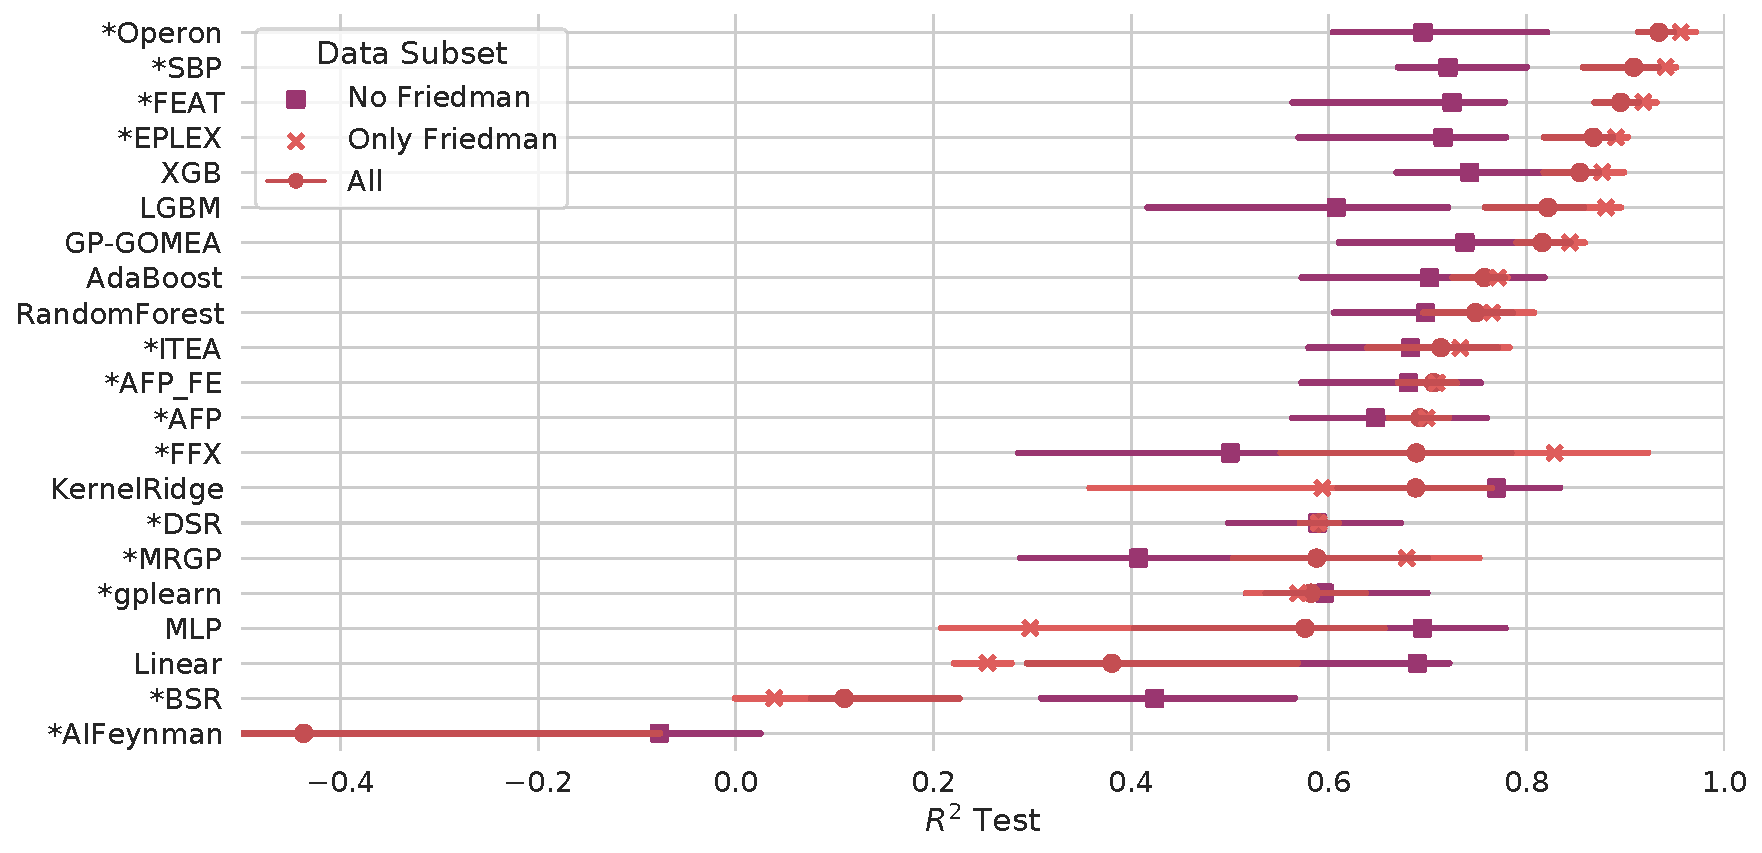
\includegraphics[width=\textwidth]{figs/results_pmlb_r1/friedman_comparison_pairgrid-pointplot_r2_test.pdf}

    \caption{
        Comparison of normalized $R^2$ test scores on all black-box datasets, just the Friedman datatasets, and just the non-Friedman datasets.
    }
    \label{fig:friedman}
\end{figure}


\subsection{Statistical Tests}
Figures~\ref{fig:heat_stats_bb}-\ref{fig:heat_stats_sr} give summary significance levels of pairwise tests of significance between estimators on the black-box and ground-truth problems. 
All pair-wise statistical tests are Wilcoxon signed-rank tests. 
A Bonferroni correction was applied, yielding the $\alpha$ levels given in each. 
This methodology for assessing statistical significance is based on the recommendations of~\citet{demsarStatisticalComparisonsClassifiers2006a} for comparing multiple estimators over many datasets.
These figures are intended to complement Figures~\ref{fig:pmlb_perf}-\ref{fig:symbolic_solns} in which effect sizes are shown. 

\begin{figure}
    \begin{minipage}{0.5\textwidth}
        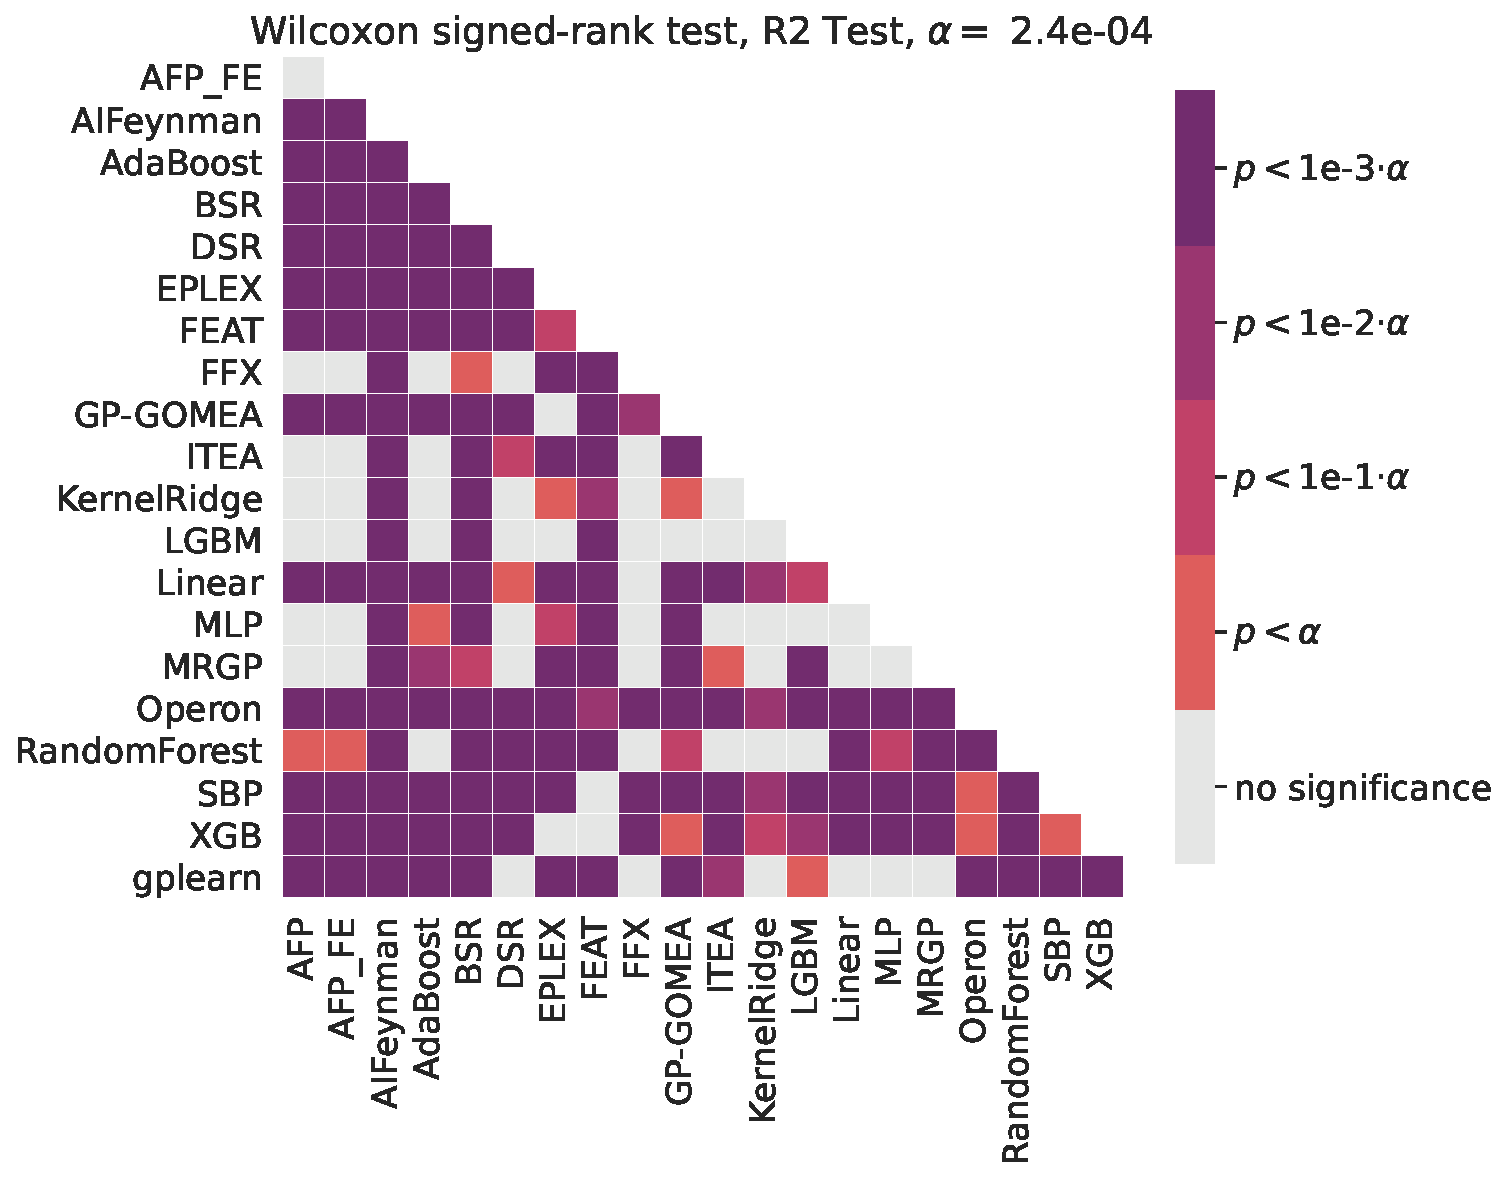
\includegraphics[width=\textwidth]{figs/Pairwise_comparison_of_R2_Test_on_black-box_problems.pdf}
    \end{minipage}
    % \hspace{0.02\textwidth}
    \begin{minipage}{0.5\textwidth}

        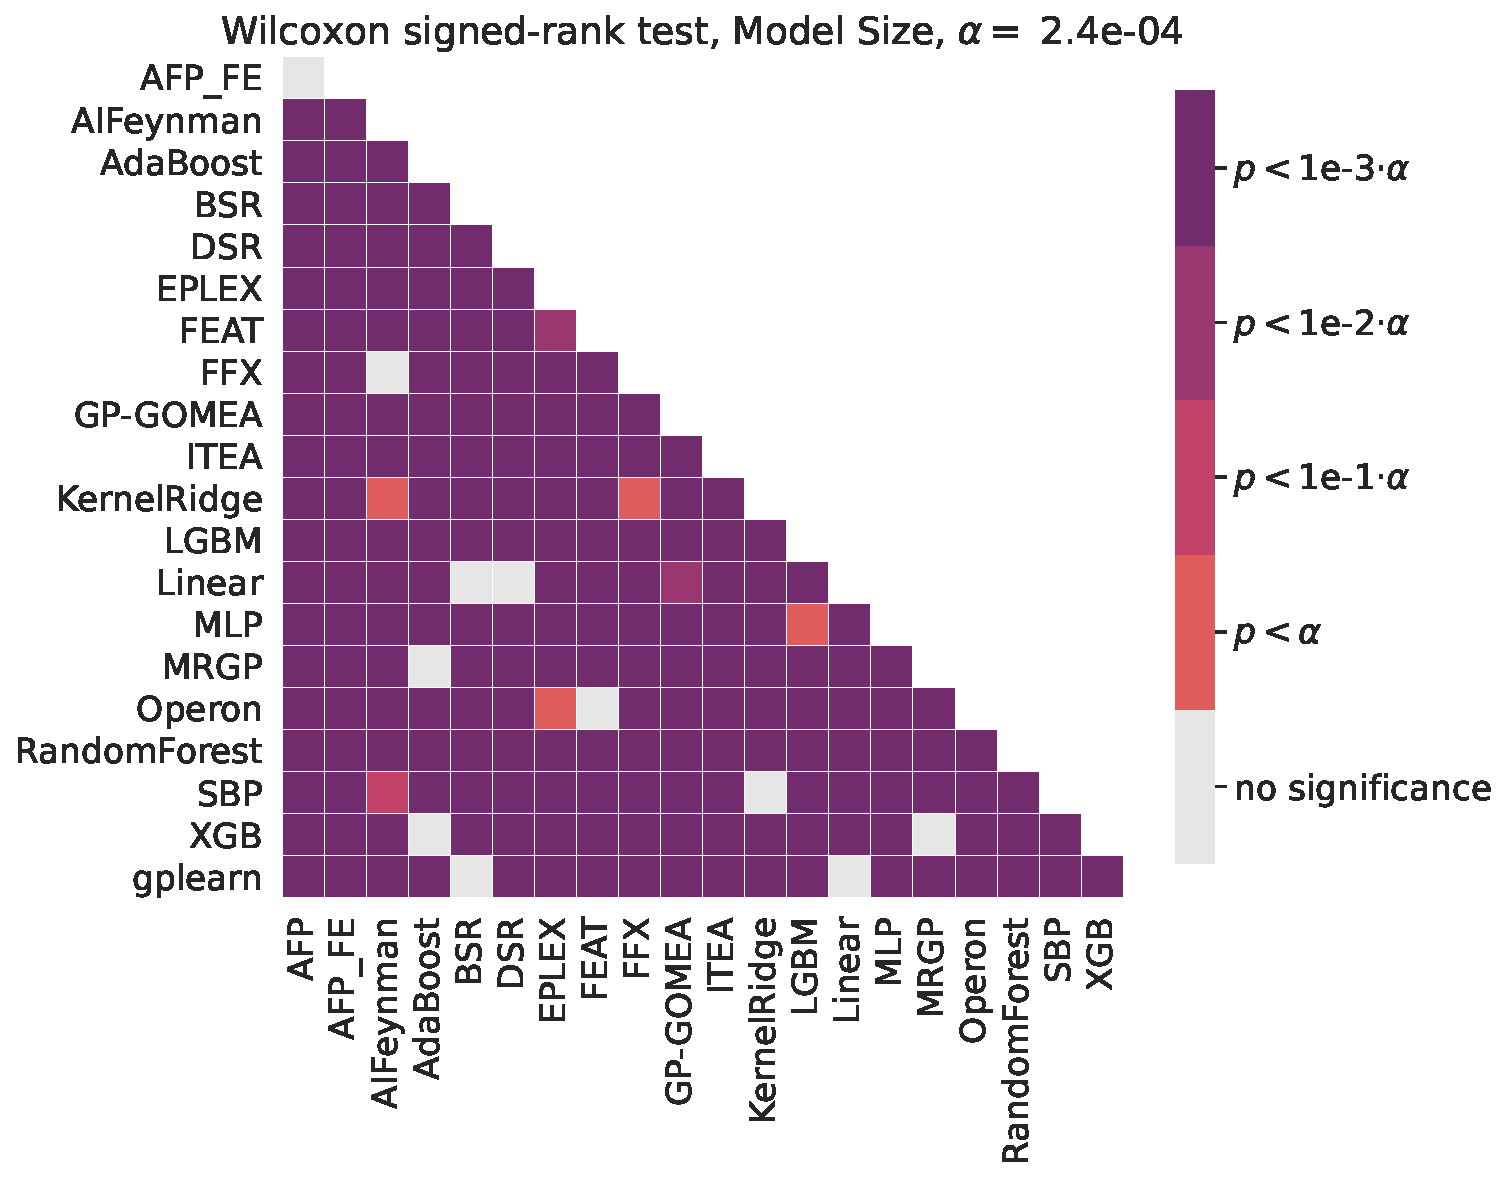
\includegraphics[width=\textwidth]{figs/Pairwise_comparison_of_Model_Size_on_black-box_problems.pdf}
    \end{minipage}
        \caption{ 
            Pairwise statistical comparisons on the black-box regression problems. 
            Wilcoxon signed-rank tests are used with a Bonferonni correction on $\alpha$ for multiple comparisons.
            (Left) $R^2$ test scores, (Right) model size. 
        }
        \label{fig:heat_stats_bb}
\end{figure}




\begin{figure}
    \begin{minipage}{0.5\textwidth}
        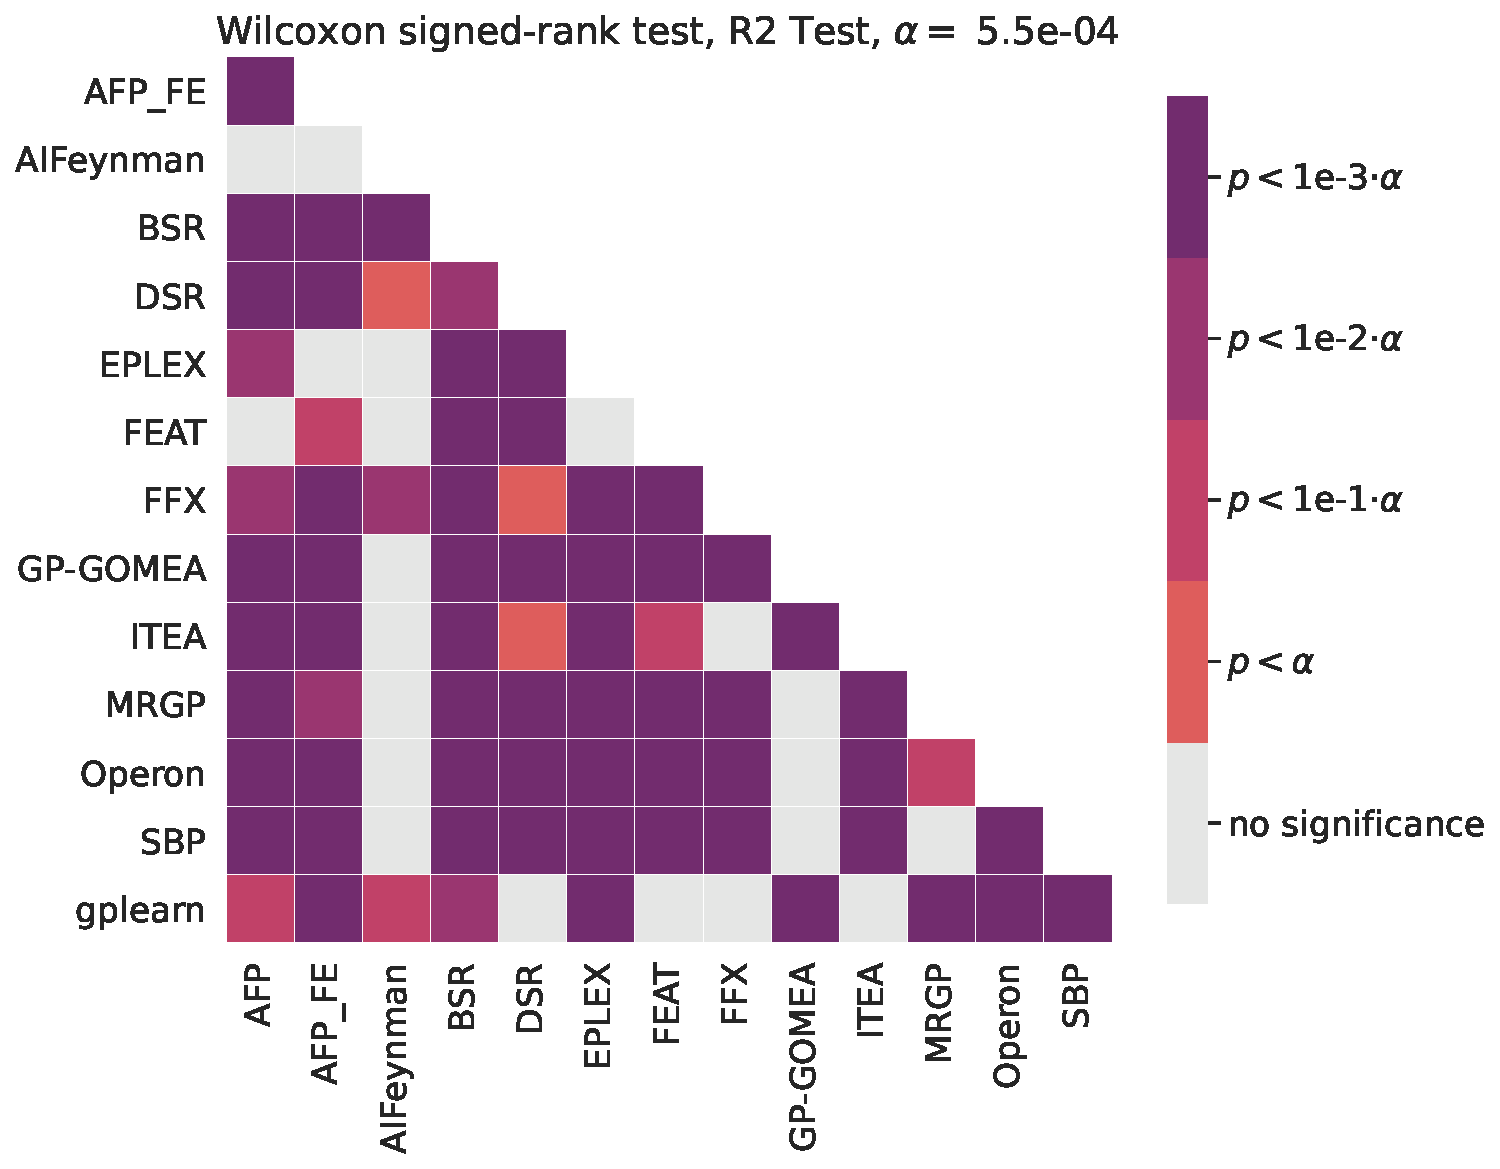
\includegraphics[width=\textwidth]{figs/Pairwise_comparison_of_R2_Test_on_symbolic_problems_target_noise=0.0.pdf}
    \end{minipage}
    % \hspace{0.02\textwidth}
    \begin{minipage}{0.5\textwidth}
        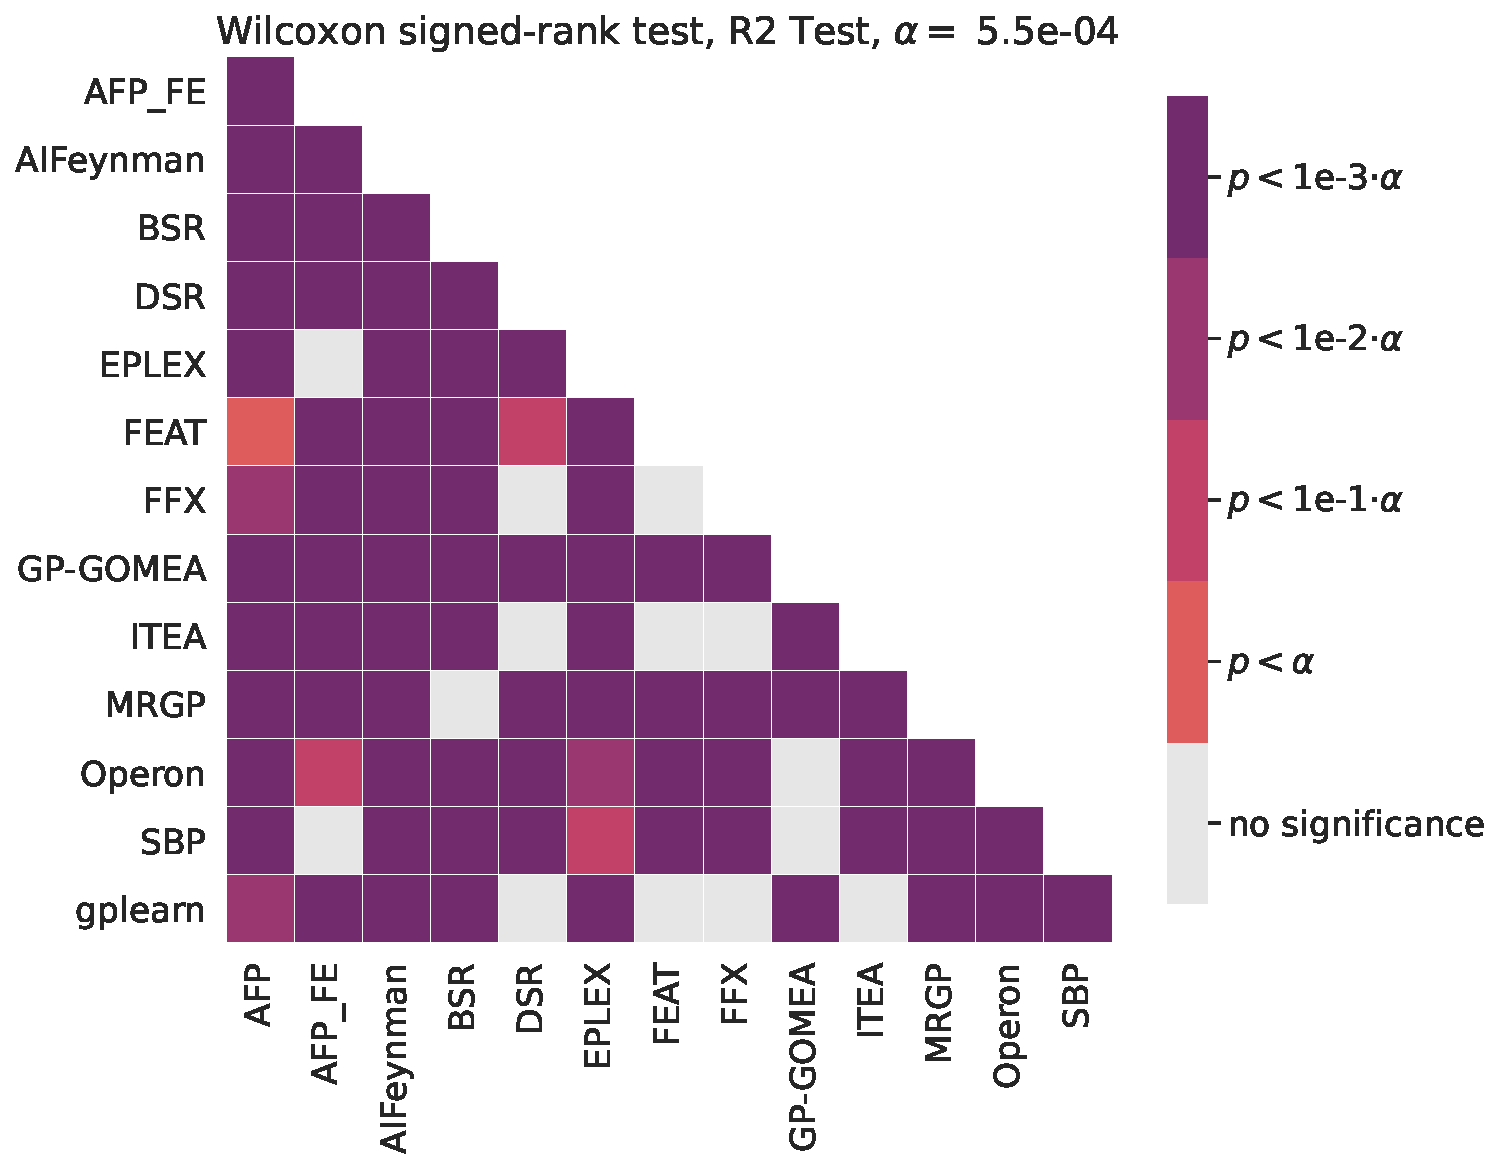
\includegraphics[width=\textwidth]{figs/Pairwise_comparison_of_R2_Test_on_symbolic_problems_target_noise=0.001.pdf}
    \end{minipage}
    \caption{ 
        Pairwise statistical comparisons of $R^2$ test scores on the ground-truth regression problems. 
        We report Wilcoxon signed-rank tests with a Bonferonni correction on $\alpha$ for multiple comparisons.
        (Left) target noise of 0, (Right) target noise of 0.001. 
    }
    \label{fig:heat_stats_r2_sr}
\end{figure}

\begin{figure}
    \begin{minipage}{0.5\textwidth}
        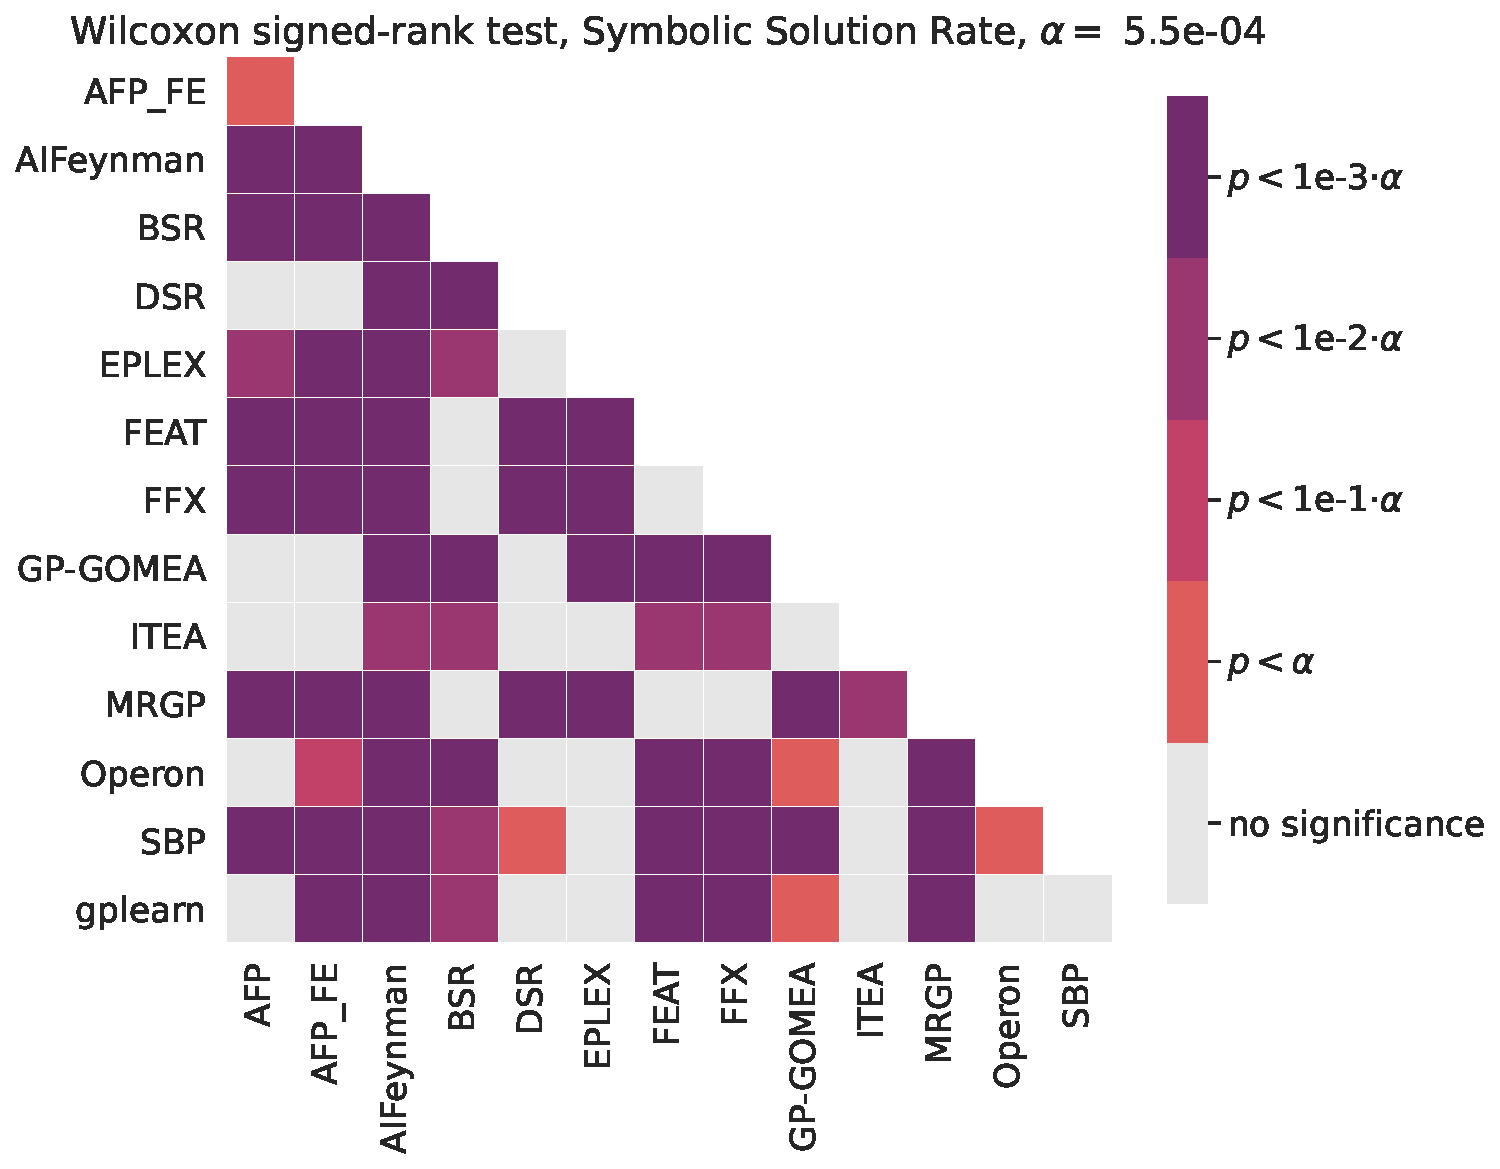
\includegraphics[width=\textwidth]{figs/Pairwise_comparison_of_Symbolic_Solution_Rate_on_symbolic_problems_target_noise=0.0.pdf}
    \end{minipage}
    \begin{minipage}{0.5\textwidth}
        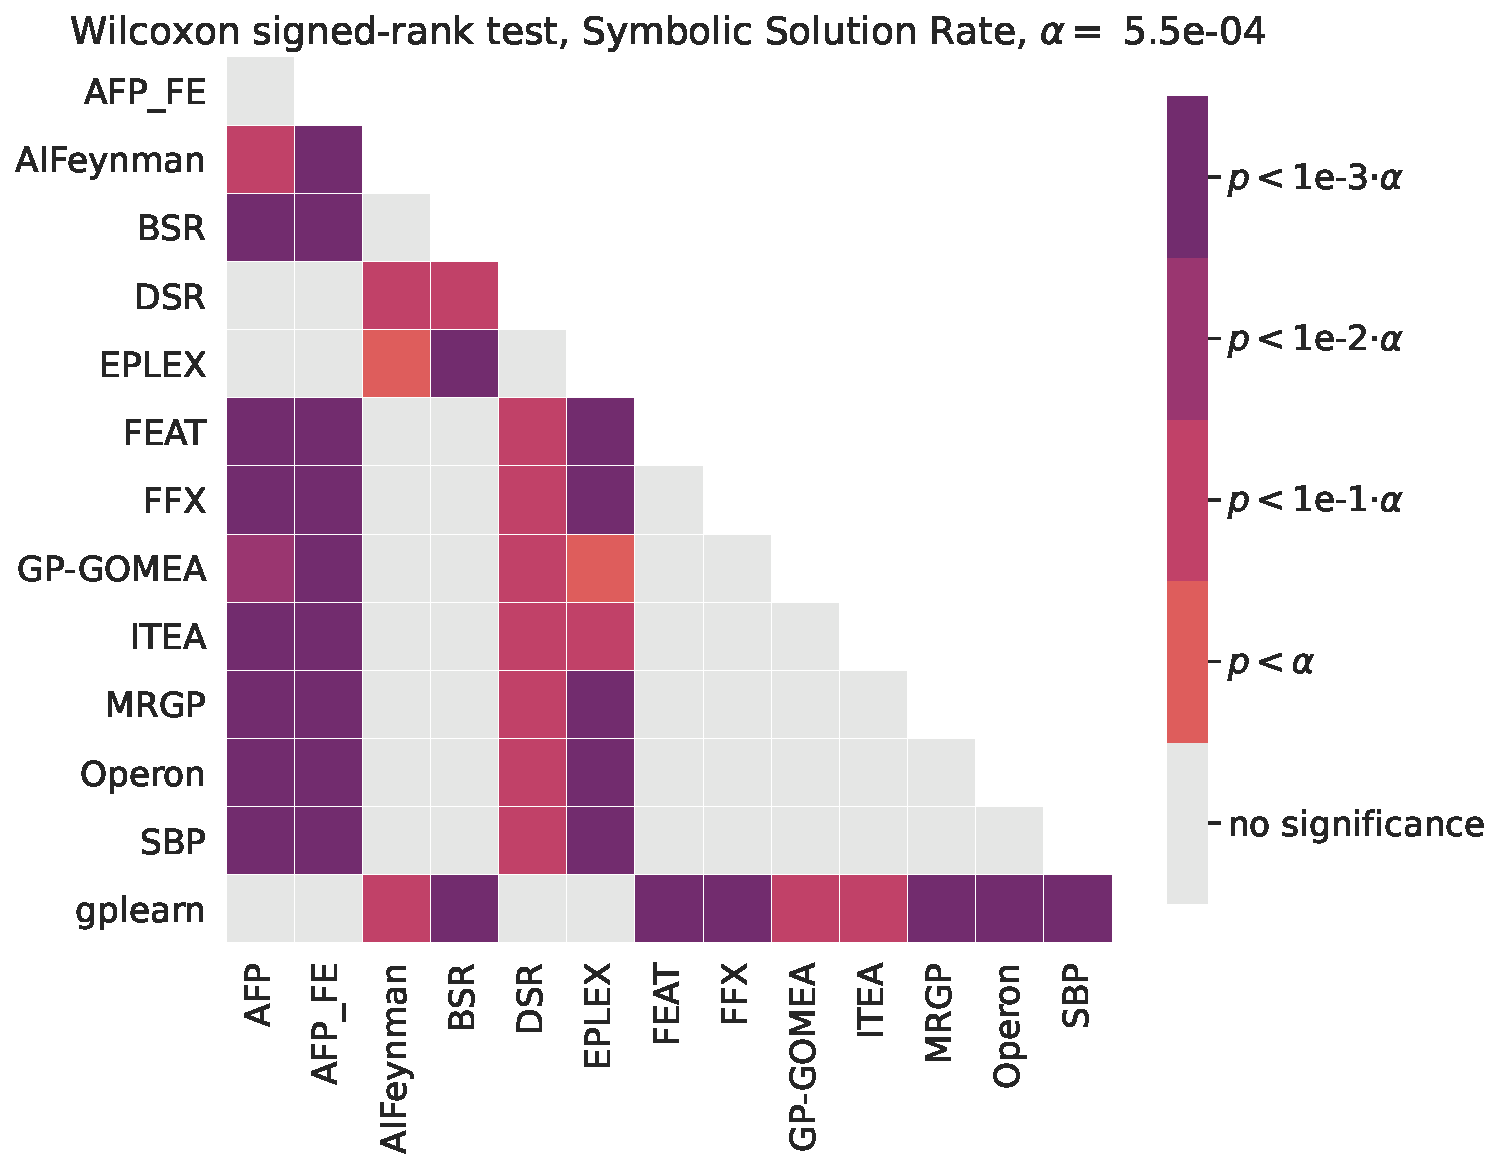
\includegraphics[width=\textwidth]{figs/Pairwise_comparison_of_Symbolic_Solution_Rate_on_symbolic_problems_target_noise=0.001.pdf}
    \end{minipage}
    \caption{ 
        Pairwise statistical comparisons of solution rates on the ground-truth regression problems. 
        We report Wilcoxon signed-rank tests with a Bonferonni correction on $\alpha$ for multiple comparisons.
        (Left) target noise of 0, (Right) target noise of 0.001. 
    }
    \label{fig:heat_stats_r2_sr}
\end{figure}

% \begin{table}
%     \centering
%     \tiny 
%     \input{tables/all_black_box_r2_test.tex}
% \end{table}
% \resizebox{\textwidth}{!}{%
% \begin{table}
\centering
\tiny
\caption{Pairwise comparisons of R2 Test across the symbolic datasets. Bold indicates significant differences ($p<\alpha$, $\alpha=$0.0005).}
\begin{tabular}{llllllllllllll}
\toprule
alg2 &           AFP\_FE &        AIFeynman &              BSR &              DSR &            EPLEX &             FEAT &              FFX &         GP-GOMEA &             ITEA &             MRGP &           Operon &              SBP &          gplearn \\
alg1      &                  &                  &                  &                  &                  &                  &                  &                  &                  &                  &                  &                  &                  \\
\midrule
AFP       &  \textbf{6.9e-31} &  \textbf{8.5e-38} &    \textbf{4e-57} &  \textbf{2.9e-46} &            0.096 &  \textbf{1.7e-21} &  \textbf{1.7e-27} &  \textbf{3.1e-25} &  \textbf{9.1e-28} &  \textbf{7.1e-33} &  \textbf{1.1e-10} &          0.00055 &  \textbf{1.8e-18} \\
AFP\_FE    &                - &  \textbf{3.8e-39} &  \textbf{1.4e-62} &  \textbf{2.9e-49} &  \textbf{3.8e-05} &  \textbf{2.3e-38} &  \textbf{4.7e-46} &  \textbf{4.6e-13} &  \textbf{1.1e-40} &  \textbf{2.6e-40} &             0.12 &            0.023 &  \textbf{9.9e-42} \\
AIFeynman &                - &                - &  \textbf{1.4e-27} &  \textbf{8.4e-36} &  \textbf{5.5e-38} &  \textbf{1.6e-34} &  \textbf{1.2e-34} &  \textbf{9.6e-42} &  \textbf{3.9e-36} &    \textbf{5e-08} &  \textbf{1.2e-38} &  \textbf{1.4e-39} &    \textbf{3e-36} \\
BSR       &                - &                - &                - &  \textbf{7.4e-30} &    \textbf{1e-53} &  \textbf{1.5e-48} &  \textbf{2.6e-53} &  \textbf{7.2e-64} &  \textbf{3.5e-41} &  \textbf{2.4e-06} &  \textbf{4.5e-60} &  \textbf{7.9e-58} &  \textbf{1.5e-24} \\
DSR       &                - &                - &                - &                - &  \textbf{8.8e-33} &             0.15 &  \textbf{2.7e-05} &  \textbf{9.3e-46} &  \textbf{1.1e-10} &  \textbf{4.2e-19} &    \textbf{2e-35} &  \textbf{3.4e-29} &  \textbf{3.5e-06} \\
EPLEX     &                - &                - &                - &                - &                - &  \textbf{3.6e-31} &  \textbf{7.9e-27} &  \textbf{2.7e-24} &  \textbf{1.9e-18} &    \textbf{6e-36} &  \textbf{8.8e-13} &  \textbf{0.00013} &  \textbf{1.7e-17} \\
FEAT      &                - &                - &                - &                - &                - &                - &            0.078 &  \textbf{2.2e-50} &            0.038 &  \textbf{1.8e-28} &  \textbf{7.3e-48} &  \textbf{1.4e-36} &            0.098 \\
FFX       &                - &                - &                - &                - &                - &                - &                - &  \textbf{9.4e-60} &             0.13 &  \textbf{2.4e-23} &  \textbf{2.3e-40} &  \textbf{5.1e-26} &             0.41 \\
GP-GOMEA  &                - &                - &                - &                - &                - &                - &                - &                - &  \textbf{3.8e-40} &  \textbf{3.8e-50} &    \textbf{6e-13} &  \textbf{3.4e-25} &  \textbf{1.3e-44} \\
ITEA      &                - &                - &                - &                - &                - &                - &                - &                - &                - &  \textbf{1.5e-21} &  \textbf{2.9e-26} &  \textbf{9.6e-18} &             0.93 \\
MRGP      &                - &                - &                - &                - &                - &                - &                - &                - &                - &                - &  \textbf{4.3e-55} &  \textbf{1.1e-47} &  \textbf{6.6e-22} \\
Operon    &                - &                - &                - &                - &                - &                - &                - &                - &                - &                - &                - &  \textbf{2.6e-45} &  \textbf{4.4e-28} \\
SBP       &                - &                - &                - &                - &                - &                - &                - &                - &                - &                - &                - &                - &  \textbf{9.3e-17} \\
\bottomrule
\end{tabular}
\end{table}

% \begin{table}
\centering
\tiny
\caption{Pairwise comparisons of Simplified Complexity across the symbolic datasets. Bold indicates significant differences ($p<\alpha$, $\alpha=$0.0005).}
\begin{tabular}{llllllllllllll}
\toprule
alg2 &           AFP\_FE &        AIFeynman &              BSR &              DSR &            EPLEX &             FEAT &              FFX &         GP-GOMEA &             ITEA &             MRGP &           Operon &              SBP &          gplearn \\
alg1      &                  &                  &                  &                  &                  &                  &                  &                  &                  &                  &                  &                  &                  \\
\midrule
AFP       &  \textbf{5.5e-10} &  \textbf{3.8e-10} &          0.00075 &  \textbf{2.4e-47} &  \textbf{1.9e-07} &  \textbf{5.2e-11} &    \textbf{7e-61} &  \textbf{2.2e-13} &  \textbf{3.6e-53} &  \textbf{5.3e-65} &  \textbf{1.1e-46} &  \textbf{3.3e-62} &  \textbf{7.4e-06} \\
AFP\_FE    &                - &  \textbf{1.3e-10} &             0.14 &  \textbf{2.4e-50} &             0.57 &  \textbf{3.9e-05} &  \textbf{1.3e-57} &           0.0069 &  \textbf{2.7e-52} &  \textbf{7.2e-65} &  \textbf{1.2e-42} &  \textbf{5.3e-62} &  \textbf{4.4e-09} \\
AIFeynman &                - &                - &  \textbf{1.5e-13} &            0.032 &  \textbf{1.3e-11} &  \textbf{7.3e-14} &  \textbf{1.3e-39} &  \textbf{1.8e-12} &             0.03 &  \textbf{2.5e-60} &  \textbf{1.4e-18} &  \textbf{1.8e-37} &            0.003 \\
BSR       &                - &                - &                - &  \textbf{3.2e-61} &           0.0047 &  \textbf{1.1e-07} &  \textbf{1.6e-59} &  \textbf{1.2e-05} &  \textbf{8.2e-62} &  \textbf{5.1e-65} &  \textbf{1.8e-42} &  \textbf{1.1e-60} &  \textbf{1.6e-09} \\
DSR       &                - &                - &                - &                - &  \textbf{1.8e-51} &  \textbf{2.8e-46} &  \textbf{3.5e-64} &  \textbf{6.7e-55} &  \textbf{0.00014} &  \textbf{2.4e-65} &  \textbf{1.9e-60} &    \textbf{4e-63} &  \textbf{7.8e-12} \\
EPLEX     &                - &                - &                - &                - &                - &  \textbf{1.9e-08} &  \textbf{4.3e-60} &             0.19 &  \textbf{4.2e-50} &  \textbf{2.7e-63} &  \textbf{1.1e-25} &  \textbf{1.4e-59} &  \textbf{1.6e-11} \\
FEAT      &                - &                - &                - &                - &                - &                - &  \textbf{1.2e-56} &           0.0093 &  \textbf{5.4e-47} &  \textbf{3.2e-58} &  \textbf{4.7e-06} &  \textbf{4.7e-52} &  \textbf{6.6e-16} \\
FFX       &                - &                - &                - &                - &                - &                - &                - &  \textbf{2.1e-54} &  \textbf{4.8e-65} &    \textbf{1e-51} &  \textbf{3.3e-44} &            0.002 &  \textbf{5.2e-53} \\
GP-GOMEA  &                - &                - &                - &                - &                - &                - &                - &                - &  \textbf{4.9e-55} &  \textbf{3.5e-65} &  \textbf{1.7e-45} &    \textbf{5e-62} &    \textbf{3e-11} \\
ITEA      &                - &                - &                - &                - &                - &                - &                - &                - &                - &  \textbf{2.3e-65} &  \textbf{5.2e-60} &    \textbf{3e-63} &  \textbf{1.9e-07} \\
MRGP      &                - &                - &                - &                - &                - &                - &                - &                - &                - &                - &  \textbf{2.3e-64} &  \textbf{1.7e-52} &  \textbf{2.5e-62} \\
Operon    &                - &                - &                - &                - &                - &                - &                - &                - &                - &                - &                - &  \textbf{9.5e-59} &  \textbf{5.7e-26} \\
SBP       &                - &                - &                - &                - &                - &                - &                - &                - &                - &                - &                - &                - &  \textbf{9.7e-53} \\
\bottomrule
\end{tabular}
\end{table}

% \input{tables/pvals_bb_r2_test.tex}
% \input{tables/pvals_bb_model_size.tex}

% \begin{table}
\centering
\caption{Pairwise comparisons of Solution Rate (%) across the symbolic datasets. Bold indicates $\alpha<$0.00055.}
\begin{tabular}{llllllllllllll}
\toprule
alg2 & AIFeynman &       BSR &       DSR &     EPLEX &      FEAT &    FE\_AFP &       FFX &   GPGOMEA &      ITEA &      MRGP &    Operon &       SBP &   gplearn \\
alg1      &           &           &           &           &           &           &           &           &           &           &           &           &           \\
\midrule
AFP       &  1.2e-65* &  1.2e-65* &  1.2e-65* &  1.2e-65* &  1.2e-65* &  1.2e-65* &  1.2e-65* &  1.2e-65* &  1.2e-65* &  1.2e-65* &  1.2e-65* &  1.2e-65* &  1.2e-65* \\
AIFeynman &         - &  1.2e-65* &  1.2e-65* &  1.2e-65* &  1.2e-65* &  1.2e-65* &  1.2e-65* &  1.2e-65* &  1.2e-65* &  1.2e-65* &  1.2e-65* &  1.2e-65* &  1.2e-65* \\
BSR       &         - &         - &  1.2e-65* &  1.2e-65* &  1.2e-65* &  1.2e-65* &  1.2e-65* &  1.2e-65* &  1.2e-65* &  1.2e-65* &  1.2e-65* &  1.2e-65* &  1.2e-65* \\
DSR       &         - &         - &         - &  1.2e-65* &  1.2e-65* &  1.2e-65* &  1.2e-65* &  1.2e-65* &  1.2e-65* &  1.2e-65* &  1.2e-65* &  1.2e-65* &  1.2e-65* \\
EPLEX     &         - &         - &         - &         - &  1.2e-65* &  1.2e-65* &  1.2e-65* &  1.2e-65* &  1.2e-65* &  1.2e-65* &  1.2e-65* &  1.2e-65* &  1.2e-65* \\
FEAT      &         - &         - &         - &         - &         - &  1.2e-65* &  1.2e-65* &  1.2e-65* &  1.2e-65* &  1.2e-65* &  1.2e-65* &  1.2e-65* &  1.2e-65* \\
FE\_AFP    &         - &         - &         - &         - &         - &         - &  1.2e-65* &  1.2e-65* &  1.2e-65* &  1.2e-65* &  1.2e-65* &  1.2e-65* &  1.2e-65* \\
FFX       &         - &         - &         - &         - &         - &         - &         - &  1.2e-65* &  1.2e-65* &  1.2e-65* &  1.2e-65* &  1.2e-65* &  1.2e-65* \\
GPGOMEA   &         - &         - &         - &         - &         - &         - &         - &         - &  1.2e-65* &  1.2e-65* &  1.2e-65* &  1.2e-65* &  1.2e-65* \\
ITEA      &         - &         - &         - &         - &         - &         - &         - &         - &         - &  1.2e-65* &  1.2e-65* &  1.2e-65* &  1.2e-65* \\
MRGP      &         - &         - &         - &         - &         - &         - &         - &         - &         - &         - &  1.2e-65* &  1.2e-65* &  1.2e-65* \\
Operon    &         - &         - &         - &         - &         - &         - &         - &         - &         - &         - &         - &  1.2e-65* &  1.2e-65* \\
SBP       &         - &         - &         - &         - &         - &         - &         - &         - &         - &         - &         - &         - &  1.2e-65* \\
\bottomrule
\end{tabular}
\end{table}

% }
% \end{table}


%SOME deleted stuff

%are represented as a list of terms and each term is a tuple containing the transformation function and a list of exponents for the polynomial equation ~\cite{defrancaGreedySearchTree2018,defrancaInteractionTransformationEvolutionaryAlgorithm2020}.
%following Eq.~\ref{eq:interaction}.
%The mutation operators can either add or remove a term, replace the exponent of a variable on a random term, create a new term through positive or negative interaction. 
%The positive interaction is the product of two interaction functions, while negative interaction is the division between two interactions. 
%performs an Ordinary Least Square to adjust the coefficients to the training set.



%Semantic backpropagation (\textbf{SBP}) is a technique invented and popularized by~\cite{wieloch2013running,krawiec2013approximating,pawlak2014semantic} to compute, for a given target value and a tree node position, what output is needed at the given position to make the output of the tree match the target value. It works by iterative inversions of the ancestry of function nodes, from the root down to the chosen node position. 
%Here, we consider the GP algorithm by~\citet{virgolinLinearScalingSemantic2019}, which is an extension of~\cite{wieloch2013running}. 
%To variate programs, SBP is performed on a random node position using the label as target, and the subtree rooted at the sampled node position is replaced with a tree chosen from a pre-computed library. 
%The chosen tree has output that best matches the one computed by SBP (i.e., using the Euclidean distance on output vectors defined over the training set), after applying the optimal affine transformation on its output.




%Symbolic model encoding

%Interaction-Transformation (IT)~\cite{defrancaGreedySearchTree2018,defrancaInteractionTransformationEvolutionaryAlgorithm2020} is another equation representation that constraints the search space to the functional forms following:
%\begin{equation}
%f(\mathbf{x}) = w_0 + \sum_{i}{w_i \cdot (t_i \circ p_i) (\mathbf{x})},
%\label{eq:appfunction}
%\end{equation}
%\noindent where $w_i \in \mathbb{R}$ are adjustable coefficients, $t_i : \mathbb{R} \rightarrow \mathbb{R}$ is the transformation function
%(e.g., $\sin, \tanh, \mathrm{sqrt}$), and $p_i: \mathbb{R}^{d} \rightarrow \mathbb{R}$ for $d$ input variables is the interaction function:
%\begin{equation}
%p(\mathbf{x}) = \prod_{j=1}^{d}{x_j^{k_j}},
%\label{eq:interaction}
%\end{equation}
%\noindent with $k_j \in \mathbb{Z}$ called the \emph{strength} of the interaction


%gene pool optimal mixin
%The goal is to prevent the disruption potentially-salient patterns of components, i.e., \emph{building blocks} with a positive concerted action.
%In~\cite{virgolin2017scalable,virgolin2020improving}, it was shown that GP-GOMEA’s linkage-based recombination works significantly better than random recombination, and is especially competitive when small, potentially interpretable solutions are sought. 
%We use the same implementation of~\cite{virgolin2020improving}.


\end{document}
